% The paper, written from the current documents alone: every formula is taken
% from docs/ALGEBRA.md (the law), docs/ENGINE.md (the engine) or
% docs/HIGHLIGHTS.md (the decisions) and cited by the name of its section, and
% every claim carries its mark (theorem, derived, computed, assumption,
% hypothesis). The paper holds no run of its own: a run enters only through the
% documents' rows. This file is the paper's source and is edited by hand.
\documentclass[11pt]{article}
\usepackage[margin=1in]{geometry}
\usepackage{amsmath,amssymb,amsthm}
\usepackage{booktabs}
\usepackage{graphicx}
\usepackage{hyperref}
\usepackage{caption}
\captionsetup{labelsep=space}
\makeatletter\@secpenalty=0\makeatother
\setlength{\abovecaptionskip}{4pt}\setlength{\belowcaptionskip}{2pt}\setlength{\textfloatsep}{12pt}
\renewcommand{\figurename}{Fig.}
\usepackage{microtype}
\usepackage{float}
\usepackage{enumitem}\setlist{nosep}
\usepackage{longtable}
\usepackage{array}
\newcolumntype{L}[1]{>{\raggedright\arraybackslash}p{#1}}

\hypersetup{colorlinks=true,allcolors=black}
\newtheorem{theorem}{Theorem}
\newtheorem{proposition}{Proposition}
\theoremstyle{definition}
\newtheorem{definition}{Definition}
\newtheorem{hypothesis}{Hypothesis}
\newtheorem{assumption}{Assumption}
\newcommand{\Z}{\mathbb{Z}}
\newcommand{\num}{\mathrm{num}}
\newcommand{\den}{\mathrm{den}}
\newcommand{\anow}{a_{\mathrm{now}}}
\newcommand{\abefore}{a_{\mathrm{before}}}
\newcommand{\anext}{a_{\mathrm{next}}}
\newcommand{\ddiv}{\ \mathrm{div}\ }
\newcommand{\dmod}{\ \mathrm{mod}\ }
\newcommand{\Wc}{W_c}
\newcommand{\bM}{\mathbf M}
\newcommand{\bD}{\mathbf D}
\newcommand{\bK}{\mathbf K}
\newcommand{\bn}{\mathbf n}
\newcommand{\claimmark}[1]{\textsc{#1}}

\title{Universe24: how a simple rule and the group of 48 arrive at Einstein and Lorentz}
\author{Alon Gonen\\
\small Independent researcher, Haifa, Israel\\
\small \texttt{alon@defounder.ai} \quad ORCID 0009-0008-2701-4599}
\date{October 2026}

\makeatletter\renewcommand\paragraph{\@startsection{paragraph}{4}{\z@}{1.75ex \@plus1ex \@minus.2ex}{-1em}{\normalfont\normalsize\bfseries}}\makeatother
\setlength{\LTpre}{6pt}\setlength{\LTpost}{6pt}
\begin{document}
\maketitle

\begin{abstract}
We state one local rule in whole numbers, Rule3, applied at every Node of a cubic lattice each interval: a second-order step of a family's level from its two levels and its six neighbours' arrivals, with integer coefficients from the family's pair and the Node's paces, and one Euclidean division whose remainder stays at the Node. Every level on the lattice is written by that one act, and everything the law says of a record is read from it: its form, which sources the fields; its Wronskian, which is the sign; and its current through a Link, Rule3's own conserved flux. On the board there are events, which split by the rule, and amplitudes, their sums at the Nodes; there is no wave and no quantum of the board's own. A click is a detector's: a detector is a declared region of Nodes, never one Node, which sees the amplitudes' current through its boundary; one wall of the quantum's action of that inflow is one quantum, and the instrument credits each quantum to one detector by the shares. That credit is the one non-local place of the description and the one thing not known; everything else is deterministic, local and bit-reversible under the rule's own direction. Exact on the lattice: the whole run returns bit for bit, a form is conserved, and the momentum's flux is the record's own stress. The families are bands of the rule. The body of nature is the cloud, the wide fixed point of the binding row, whose three masses (the well it sources, the quanta it resists with and the tail it falls with) are one to the order $(C / \Gamma)^2$; the compact pixel is collapsed matter. From the same coefficients, with a held level lowering the clock's pace once and the Link's pace once more, come the gravitational redshift, light's bending by twice the clock's share, the delay, the perihelion's $6\pi$ once the clock carries its second order, and Lorentz's factor at a body's own light speed; each form stands on the comparison side and none is an input. The paper carries two experiments and no more, each a run of the engine against a blind row written first: the two slits, whose screen of twelve declared detectors gives the fringes at the near field's places, $284$ clicks against the blind $273$, and with one gap closed one gap's envelope as in nature; and Bell, where a pair laid as one record and read by a declared two-port detector per side gives nature's $E = \cos(\delta_A + \delta_B)$ and $S = 2.76$ among the coincidences at the detector's efficiency $0.64$, and $S = 2.00$ exactly when every quantum is counted: the excess is the detection loophole and not the law, and nature's loophole-free runs at efficiencies above $0.83$ are where the law and nature part. The paper claims that the detectors' clicks represent reality and shows the match; it never claims that nature is so. To go further it needs experiments designed for one thing: to learn how nature's click patterns are turned into the law's parameters and families; the first number so fixed is the vacuum content, $0$.
\end{abstract}

\noindent\textbf{Keywords:} integer lattice model; one local rule; the click as the measurement; locality; discrete relativity; pre-registered simulation

\section{Introduction}\label{sec:intro}

\paragraph{The question.} The law of this paper is one line of integer arithmetic applied at every Node of a cubic lattice at every interval. Nothing else acts: no field equation beside it, no law of motion for a body, no rate, no draw, no real number. The paper states that line, proves what is exact on the lattice, derives what follows from the line alone, names what is decided beside it, and sets the law's own numbers beside the forms of nature: the forms of Einstein, Lorentz, Newton, de Broglie and Young appear only on the comparison side, beside the law's expectation written before any run; none is an input. The group of the title is the $48$ signed permutations of the three axes, the cube's full symmetry group, its $24$ rotations with their reflections, under which the law is covariant with the translations; Einstein and Lorentz in the title are their forms, the weak field's bending, delay, redshift and perihelion and Lorentz's factor for a moving clock, arrived at from the rule's coefficients and never its equations or its group as inputs. Every formula is taken from the law's document \cite{algebra} and cited by the name of the section it stands in; the engine that computes the rule is described by its own document \cite{engine}, and the decisions in force by theirs \cite{decisions}.

\paragraph{The click's story, the spine of the paper.} On the board there are events and amplitudes: an emitter's events, declared in a file or written by a body, split by Rule3 to the six neighbours at every Node, every possibility at once, and the amplitudes are their sums at the Nodes, the record. Nothing on the board is a wave and nothing on the board is a quantum: the record is deterministic, bit-reversible, and never ends. A click is a detector's. A detector is a declared region of Nodes, never one Node, at least half a wavelength across (no click names a Node: a quantum with a direction has no Node), which sees the amplitudes' current through its boundary; the quantum's action measures that inflow, so the detector saw $N$ quanta where its inflow over the passage is $N$ walls; and the instrument credits each quantum to one detector, by the shares of the inflows over every declared detector, one click per quantum and never two (Section~\ref{sec:detector}). The credit is a declaration of the instrument and no line of the law: the law gives the shares, and no line of it gives, exactly, at which detector a quantum falls. That is the one non-local place of the description and the one thing the paper does not know; it is stated once here and never contradicted. The record goes on after the click; what a detector absorbed leaves the declared board through the face that backs it and no echo returns; the other possibilities go on as empty amplitudes, in no click (Section~\ref{sec:nothing}). The count's line and the sense's line, under which the paper's earlier drafts moved whole quanta and the sign between Nodes by a division at every Node, left the law at the owner's word of 2026-10-01: the physics reads the record alone, the form for the wells, the Wronskian for the sign and the current for what a detector sees (Section~\ref{sec:left}). The price of locality is stated plainly in Section~\ref{sec:price}: exclusivity and Born's rule are the instrument's and no finding; a detector in one gap of the two slits that absorbs is the closed slit; and Bell's correlation is reached only through a detector whose credit depends on the pair's phase, the detection loophole, so that where nature closes the loophole the law and nature part. A finding against nature is a click compared with a click, nothing else: where a click row of the law stands beside a click row of nature's and differs, the paper writes it as it stands; a number computed from the algebra and set beside nature's number is a computation, marked so; and a GameBoard reading is never compared with nature.

\paragraph{The reading rule.} Inside is inside the GameBoard, where no one measures; Outside is the game above the board, the detectors and their clicks. Only a detector's click is a measurement, compared with nature or pinned as an expectation. A number of the GameBoard's state (a level, a support, a total, a body's centre, a region's inflow before the credit) is a GameBoard reading, a diagnostic, labelled so wherever it appears, never compared with nature and never a result on its own; a number whose kind is not named is not a result. So clicks are compared with clicks: nobody measures the board, and a finding against nature is a click row of the law beside a click row of nature's, never a reading of the board and never a computation on its own \cite[readings and measurements; the reading]{algebra}\cite[only clicks against clicks]{decisions}. The paper names no wave on the board: where nature says a wave the paper says an emitter's events that spread and a detector that measures them or not, and between the two ends events and amplitudes; where nature says a plane wave it says a plane record, the record of one wave number; interference is split events meeting with opposite signs (Section~\ref{sec:nowaves}). What produces a click is not known and not claimed: everything on the board is deterministic, a human measures only realised events, and the detector's declaration stands in the place of a mechanism, as nature's detectors are described by what they report and not by why \cite[what produces a click is not known]{algebra}\cite[what produces a click is not known]{decisions}. The paper claims that the Outside represents reality and shows the match; it never claims that nature is so \cite[inside and outside]{decisions}.

\paragraph{The marks.} Every claim carries one of five marks: \claimmark{theorem}, proved for every GameBoard; \claimmark{derived}, from theorems by argument; \claimmark{computed}, a number of the law's own computed from its lines before any run; \claimmark{assumption}, a line the law holds by decision and names where it is used; \claimmark{hypothesis}, a line outside the law under its own name, with what would decide it. A number of a run enters only through the documents' rows, labelled \textsc{detector} (a click, the measurement) or \textsc{gameboard} (a diagnostic).

\paragraph{The law in one line.} At every Node, each interval, for every family \cite[the line; the booking; the primitives]{algebra}:
{\small\begin{equation}\label{eq:law}
\boxed{\begin{aligned}
&\text{Rule3:} && w\,\anext + r' = \textstyle\sum_{a \in \{x, y, z\}} R_a\,(\mathrm{arr}_{+a} + \mathrm{arr}_{-a}) + S\,\anow - w\,\abefore + r, \quad 0 \le r' < w,\\
&&& w = 6\,\den\,\Gamma^2, \quad R_a = 2\,\num\,p_a^2,\\
&&& S = 12\,\den\,\Gamma^2 - 12\,(\den - \num)\,p_0^2 - 4\,\num\,(p_x^2 + p_y^2 + p_z^2);\\
&\text{the one write:} && \text{a level at a Node gains } (w\,q(\text{Node}) + r) \ddiv E, \text{ the remainder } r \text{ kept there};\\
&\text{the readings:} && D_i = \mathrm{now}_i^2 - \mathrm{next}_i\,\mathrm{before}_i, \qquad W_i = \mathrm{re}_{\mathrm{now}}\,\mathrm{im}_{\mathrm{before}} - \mathrm{im}_{\mathrm{now}}\,\mathrm{re}_{\mathrm{before}},\\
&&& F_{ij} = \num\,(\mathrm{now}_i\,\mathrm{before}_j - \mathrm{before}_i\,\mathrm{now}_j).
\end{aligned}}
\end{equation}}
In the first line $\anow$, $\abefore$ and $\anext$ are the family's level at the Node now, one interval before and one interval on; $\mathrm{arr}_{\pm a}$ is the arrival through the Port $\pm a$, the neighbour's level; $r$ and $r'$ are the remainder kept at the Node before and after the step; $\Gamma$ is the Node clock, the pace of an empty Node; $[\num, \den]$ is the family's pair, with $\cos\omega_0 = \num / \den$ its rotation per interval at wave number zero; $p_0$ is the Node's clock pace and $p_a$ its pace along the axis $a$, both the Node clock lowered by the levels the family reads there; and $\ddiv$ is the floor division. The second line is every write of a record into a held level: $q(\text{Node})$ is the writer's own quantity there, $w$ the one weight with which the writer's family reads the written family, and $E$ the written row's divisor. The third line is what is read from a record and never written: its form $D_i$ at a Node, whose quotient over the quantum's action $T$ is the well that sources the fields; the Wronskian $W_i$ of its two level pairs, the sign; and its current $F_{ij}$ into the Node $i$ from its neighbour $j$ over the interval, Rule3's own conserved flux, which a declared detector sees through its boundary and which the instrument counts in quanta, one per wall $\Wc = 3\,\den\,T$ of inflow. Everything else is a number in a file. The first line is a theorem's object (Section~\ref{sec:rule}), the second the one write (Section~\ref{sec:write}), the third the click's (Section~\ref{sec:click}).

\paragraph{The words.} The physical location is a \emph{Node}; its complete local information is its \emph{NodeState}, the law's own numbers and nothing else. Nodes are joined by \emph{Links} through six directional \emph{Ports} per Node; the lattice of Nodes is the \emph{GameBoard}; a local change is an \emph{Event}, and there is one \emph{LocalRule}, Rule3. A \emph{Family} is one kind of physical value with its pair and what it holds; its \emph{Record} is its levels over the GameBoard, two per Node with a remainder. A \emph{Body} is the Nodes on which a family's record stands bound, its quanta the record's share, with no law of its own; a \emph{Message} is a record the world lays and no body, an emitter's events. A \emph{Detector} is a region of Nodes declared in the file to report, a declared instrument; its \emph{Click}, one quantum credited to it by the instrument from the current it saw through its boundary, is the one measurement, reported with the region, the family and the Ports crossed and never a Node. An \emph{Interval} is one step of the whole GameBoard \cite[the objects]{algebra}\cite[the words]{engine}.

\begin{figure}[!tb]\centering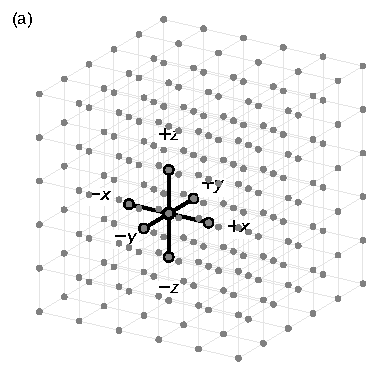
\includegraphics[width=0.36\linewidth]{figures/lattice.pdf}\caption{\label{fig:lattice}The GameBoard in space: a cubic array of Nodes, here $6 \times 6 \times 6$, each joined to its six neighbours by Links through the Ports $\pm x$, $\pm y$, $\pm z$ (the faint lines); one Node and its six neighbours marked, the Nodes one interval away from it, whose convex hull is the octahedron of Fig.~\ref{fig:octahedron}. A Node keeps each family's two levels and its remainders there, and nothing else. Drawn from the definitions; no run.}\end{figure}

\paragraph{What this paper claims, and what it does not.} Claimed: one explicitly stated integer rule whose reversibility, conserved form and momentum's flux are theorems on the lattice; the click as a declared detector's reading of the record's own current, the record never ending, with the one non-local place named; the families as bands of that rule; the cloud as the body of nature with its three masses one, and the compact pixel as collapsed matter; the forms of nature arrived at from the coefficients and set beside their known forms; and two experiments run against blind rows, the two slits and Bell, each written as it stands. Not claimed: that nature is so; a derivation of the Lorentz group, which is no symmetry of the lattice (the lattice's symmetries are the 48 signed permutations of the axes); a mechanism of the click; Bell's correlation at a fair sample, which the law reaches only through the detection loophole; the fine-structure constant, the mass ratio of the proton to the electron or what fixes the Node clock, which are open by name (Section~\ref{sec:open}). The paper holds no run of its own; every number of a run is the documents' and is cited so.

\section{The general formula}\label{sec:rule}

This section states the object and proves what is exact on it: the lattice and its families, the one line with its coefficients, its reversibility, what its acts can and cannot form, the paces with their guard, the conserved form, the tension as the wave's own stress, the one write, the interval and its inverse, and the three channels through which one family acts on another \cite[the GameBoard and the families; Rule3; the primitives]{algebra}.

\subsection{The objects}\label{sec:objects}

A Node is a physical location. The GameBoard is all the Nodes together, a box of $(N_x, N_y, N_z)$ Nodes; each axis is periodic (the box a torus on that axis), open (a face beyond which no Node lies, read as $0$) or folded (an axis of one layer, whose two Ports return the Node itself), as the world declares. Two Nodes that differ by one step along one axis are joined by a Link; each Node has six Links, one through each of its six Ports, $\pm x$, $\pm y$, $\pm z$ (Fig.~\ref{fig:octahedron}). An inner face is the face's rule declared inside the board: a plane of Nodes across an axis, beyond the board but for the gaps the world declares; a Node beyond the board is read as $0$ through every Port and reads $0$ through its own (a held row with a declared rest is read at its rest there, $0$ since the vacuum content is $0$, the vacuum beyond the face being the same vacuum), so no level, current or source crosses its Links, and no body, message or detector stands there. The board's shape is a declaration of the file, like the wraps and the detectors' regions, and no number of the engine. A face may also be declared receding (\claimmark{assumption}, the owner's decision, built): the board is a dense cube that grows by a layer of zeros on that side whenever a level other than $0$ reaches the Node before the face, so no event ever meets it, and a run of such a board is a run of the unbounded lattice with $0$ beyond the front, since Rule3 needs nothing else and a level leaves $0$ only where a neighbour was not $0$ the interval before; an option beside open, folded and periodic faces, never the default, with a declared largest size at which a run reports and ends; on it the massless and the binding rows build their rest behind the front by the run itself (Huygens on the lattice, within $3$ percent in ten intervals), nothing reflects, the blind numbers of the looks are the infinite lattice's exactly, and the world's size is its age in Links; a receding face grows the board and stretches nothing, so Hubble's redshift does not come from the law's growth \cite[the unbounded board]{algebra}\cite[the receding face]{decisions}. The local information of a Node is its NodeState: the levels and remainders of the families at that Node, the held rows' carries, and nothing else; no register, no table, no formula and no draw stand at a Node \cite[the objects]{algebra}\cite[nothing at a Node but the law's numbers]{decisions}.

A family is one kind of physical value with its own declarations: its pair $[\num, \den]$ and what it holds. Its record is two levels per Node (now and before) with a remainder per Node; a family of quanta carries two such level pairs, the real one and its second, the rotation sense (Section~\ref{sec:sign}). A body is a set of Nodes on which a family's record stands bound, one connected region, its quanta the record's share there (Section~\ref{sec:bodies}); a message is a record the world lays and no body, a packet of a family of quanta with its axis, its wave number, its amplitude and its envelope declared \cite[the objects]{algebra}.

\begin{figure}[!tb]\centering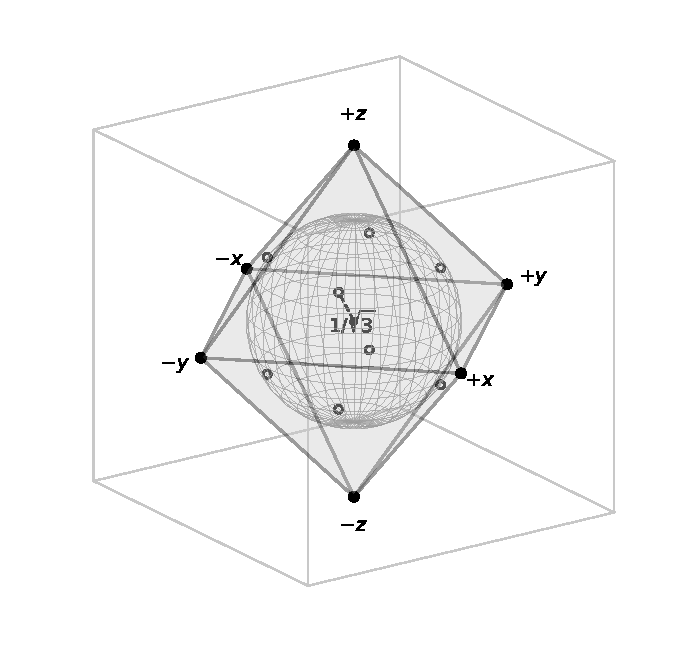
\includegraphics[width=0.30\linewidth]{figures/octahedron.pdf}\caption{\label{fig:octahedron}The six Ports of one Node, $\pm x$, $\pm y$, $\pm z$, and the octahedron they span: the Nodes one interval away. The maps of the six Ports onto themselves that keep opposite Ports opposite are the $48$ signed permutations of the axes, the symmetry group of the cube, under which the law is covariant. Drawn from the definitions; no run.}\end{figure}

\subsection{The line}\label{sec:line}

At every Node, each interval, every family steps by the first line of Eq.~\eqref{eq:law}: the six arrivals, each the neighbour's level through its Port ($0$ beyond an open face, the Node's own level on a folded axis), the Node's own level now, minus its level before, plus the remainder kept at the Node, divided once by the wall $w$; the quotient is the next level and the remainder stays. The remainder is the Node's own and never travels \cite[the line]{algebra}.

At the vacuum's pace $p_0 = p_a = \Gamma$ the self coefficient vanishes and the line is the plain second-order wave rule of the pair,
\begin{equation}\label{eq:vacuum}
\anext + \abefore = \frac{\num}{3\,\den}\sum_a (\mathrm{arr}_{+a} + \mathrm{arr}_{-a}),
\end{equation}
whose rotation at the wave vector $\mathbf k$ is $\cos\omega = \frac{\num}{3\,\den}\sum_a \cos k_a$: at wave number zero $\cos\omega_0 = \num / \den$, and for the massless pair $[1, 1]$ along one axis $\cos\omega = (2 + \cos k) / 3$, so that $\omega = |k| / \sqrt 3$ as $k \to 0$. Light's speed at long wavelength is therefore $1 / \sqrt 3$ Links per interval, under the causal bound of one Link per interval, the arrival's own speed; the two differ, and what in nature is one Link and one interval rests on the units of Section~\ref{sec:constants} \cite[the lattice constants]{algebra}.

\paragraph{The clock once and the Link twice.} From the coefficients, the rotation at a Node of the clock's pace $p_0$ and the Link's paces $p_a$ is (\claimmark{derived})
\begin{equation}\label{eq:bandpace}
\cos\omega = 1 - \Bigl(1 - \frac{\num}{\den}\Bigr)\Bigl(\frac{p_0}{\Gamma}\Bigr)^2 - \frac{\num}{3\,\den}\sum_a \Bigl(\frac{p_a}{\Gamma}\Bigr)^2 (1 - \cos k_a),
\end{equation}
the mass term scaling with the clock's square and the band term with the Link's pace. Two readings follow and no third \cite[the clock once and the Link twice]{algebra}. (i) \emph{The clocks shift alike}: at $k = 0$ every massive band's rest rotation obeys $1 - \cos\omega_b = (p_0 / \Gamma)^2 (1 - \cos\omega_0)$, one factor for every family, so two bound bodies at one Node shift their clocks alike, and a packet's fall in a pace gradient does not depend on its family beyond its band's own shape. (ii) \emph{The Link is twice}: along a Link every wave's speed falls with $p_a = \Gamma - 2c - t_a$, the held level $c$ entering the Link twice and the clock once, so light, which reads the held rows as every family does, is delayed and bent by twice the clock's share (Section~\ref{sec:forms}). The line is not conformal: a light wave at a fixed wave number scales with $(p_a / \Gamma)^2$ and a bound mode at rest with $(p_0 / \Gamma)^2$, and the two differ already at first order in $c / \Gamma$.

A held family's field steps at its row's pair with the pace $1$ and the wall $3\,\den$, at first order: for the massless row $\anext = (S_6(\anow) - 3\,\abefore + r) \ddiv 3$, $S_6$ the sum over the six neighbours, and for a row with a gap $3\,\den\,\anext + r' = \num\,S_6(\anow) - 3\,\den\,\abefore + r$, the same call at the row's own pair \cite[the vacuum's row steps at the divisor 1]{algebra}.

\subsection{The direction}\label{sec:direction}

Let $\sigma$ be the direction, $+1$ forward and $-1$ backward, let $\ddiv$ and $\dmod$ be the floor division and its remainder in $[0, w)$, and let $\rho$ be the remainder carried in. With
\begin{equation}\label{eq:direction}
u = \sigma\Bigl(\sum_a R_a\,\mathrm{arr}_a + S\,x - w\,y\Bigr) + \rho, \qquad z = \sigma\,(u \ddiv w), \qquad \rho' = u \dmod w,
\end{equation}
forward $(x, y, \rho) = (\anow, \abefore, r)$ gives $(z, \rho') = (\anext, r')$, and backward $(x, y, \rho) = (\anow, \anext, r')$ gives $(z, \rho') = (\abefore, r)$.

\begin{theorem}[the direction]\label{th:direction}
The backward call returns $(\abefore, r)$ bit for bit; the reversibility of every step needs no second function.
\end{theorem}

\begin{proof}
Forward, $\sigma = 1$, the line is the definition of $\ddiv$ and $\dmod$. Backward, $\sigma = -1$: write $Y$ for the right side's first two terms, $\sum_a R_a\,\mathrm{arr}_a + S\,\anow$. Then $u = w\,\anext - Y + r'$ and $z = -\lfloor u / w \rfloor = \lceil (Y - w\,\anext - r') / w \rceil$. From the forward line, $Y - w\,\anext - r' = w\,\abefore - r$ with $0 \le r < w$, whose ceiling divided by $w$ is $\abefore$ exactly; and $\rho' = u - w\lfloor u / w \rfloor = w\,\abefore - (Y - w\,\anext - r') = r$. Checked bit for bit on $20{,}000$ random cases against a forward and a backward function written separately \cite[the direction]{algebra}.
\end{proof}

\subsection{The four acts and what they can form}\label{sec:acts}

Rule3's line is one act; declared coefficients make it four: (a) the read, the line over the GameBoard with its six arrivals; (b) the one-Node step, the line with the neighbours' reads declared $0$, $\anext + \abefore = (a / b)\,\anow$, the rotation by the angle whose doubled cosine is $a / b$ (Chebyshev's recurrence), which with $a / b = 1$ and the coefficient on $\abefore$ declared $0$ keeps a level and with $a / b = 2$ from $(0, 1)$ counts; (c) the division, the line with $R = S = 0$, Euclid's division with the remainder kept; (d) the load, a declared integer in the numerator, how a count enters a level. A composition of the acts is a finite sequence of them, each with its coefficients declared in the files, applied to declared levels \cite[the four acts]{algebra}.

\begin{theorem}[what the acts can form]\label{th:acts}
Every composition of the four acts is a piecewise-linear function of the levels with integer slopes: a sum of linear forms and of floors of linear forms, composed. No such function is quadratic in the levels.
\end{theorem}

\begin{proof}
Each act is a linear form of the levels or the floor of one; a floor of a linear form is piecewise linear with integer slopes; sums and compositions of such functions are of the same kind. The second difference of such a function in any one level is $0$ almost everywhere, while the second difference of a product $\mathrm{now}_i\,\mathrm{before}_j$ in the pair $(\mathrm{now}_i, \mathrm{before}_j)$ is $1$. So nothing bilinear comes from the acts alone.
\end{proof}

What the theorem separates: every product of two levels in the engine is a \emph{booking}, a reading of a bilinear form with declared coefficients and no write (Section~\ref{sec:booking}); the three bookings the law reads are the form, the Wronskian and the current, and the current is Rule3's own conserved flux (Section~\ref{sec:form}). Nothing on the board is written from a product; a detector's reading of the current is the host's and writes nothing.

\paragraph{The three tests and the six verbs.} A line enters the law only if it is generic (one primitive with declared integers, no family's name and no kind), vector (one of the acts on the state, no root and no float) and local (its own record and the six neighbours, nothing kept at a Node beyond the law's numbers); a hypothesis that needs more is stated under its own name, outside the law. Every integer of the law is made of six operations only: the translation of an accumulator by its rate, the bilinear form with a declared matrix, the group-ring addition, the permutation, the evaluation at the primitive root of unity, and the Euclidean division with the remainder kept; a root, a true division or a draw is outside the law. No act of the interval takes a square root: the integer square root stays only at load and in the generator, as the fixed point of the division act iterated, $x \leftarrow (x + n \ddiv x) \ddiv 2$ from above until it repeats \cite[the three tests of every rule]{algebra}\cite[the six verbs; the root leaves everywhere]{decisions}.

\subsection{The paces and the guard}\label{sec:paces}

The pace of a Node for a family is what its reads make of the Node clock:
\begin{equation}\label{eq:paces}
p_0^2 = (\Gamma - c)^2 + c^2, \qquad p_a = \Gamma - 2c - t_a, \qquad c = \sum_{\text{reads}} \text{weight} \times \text{by} \times \text{the read family's time level},
\end{equation}
$t_a$ the axis content from the read families' tensions on the axis $a$ (each $\text{weight} \times \text{by} \times \text{the } aa \text{ part} \ddiv 2$, one division per read per axis, rounded at the read since the pace is a coefficient and no level). A positive weight is a hollow (the read family's level slows the clock, an attraction); a negative weight is a hill. By sign the weight is multiplied by the reader's $q$ at the Node, the sign of its own rotation sense there (Section~\ref{sec:sign}). A family with no reads steps at $p_0 = p_a = \Gamma$, the plain rule. The clock's slowing is this pace: a record at a Node of pace $p$ rotates and moves as a record at $\Gamma$ does, with its intervals $p / \Gamma$ as long. Every family of quanta reads every holder of the content at the weight $1$, a row without a gap and a row with a gap alike as its stepped field, $x = (L_b + L_g) / \Gamma$ with $L_b$ the binding holder's level and $L_g$ gravity's, and every holder of the sign by its own $q$; a family sources what it reads at the weight it reads with \cite[the paces; the reads are the held row's pair's]{algebra}.

\paragraph{The clock's second order is the composition.} Each unit of the level slows the clock as it already stands, $p_0 = \Gamma (1 - 1 / \Gamma)^c$, whose square to the second order is $(\Gamma - c)^2 + c^2 = \Gamma^2 (1 - 2\Phi + 2\Phi^2)$ in the level's share $\Phi = c / \Gamma$; Rule3's coefficients take the paces' squares as written, with no division act, no rounding and no root, and $p_0 = \Gamma - c + c^2 \ddiv 2\Gamma$ to the unit is a reading of the algebra; the Link's pace stays $\Gamma - 2c - t_a$, the level entering it twice \cite[the clock's second order is the composition]{algebra}. Section~\ref{sec:forms} reads the perihelion off this second order.

\paragraph{The guard, on squares, once at load.} $0 < p_a$ and $p^2 (\den + \num) \le 2\,\den\,\Gamma^2$ at every Node, with the edge's square $P^2 = 2\,\den\,\Gamma^2 \ddiv (\den + \num)$, $\Gamma^2$ for light and above it where $\num < \den$, read on the clock's square and on each Link's pace alike over the whole initial state and never in the interval. Below $0$ a pace is no clock; beyond $P$ the step is unstable: the mode at wave number $\pi$ on every axis has the factor $2 - 2(1 - \num / \den)(p_0 / \Gamma)^2 - 4(\num / \den)(p_a / \Gamma)^2$, which is $-2\,\num / \den$ in the vacuum and stays at or above $-2$ wherever $p_0$ and $p_a$ are both at or below $P$, since $(P / \Gamma)^2 (2 - 2\num / \den + 4\num / \den) \le 4$ exactly when $P^2 (\den + \num) \le 2\,\den\,\Gamma^2$ (\claimmark{theorem}). In the run no act reads a Node to refuse: every coefficient is a square, $R_a = 2\,\num\,p_a^2$ passes through $0$ as the content reaches $\Gamma \ddiv 2$ (the Link closes: the horizon) and reopens mirrored beyond it, and beyond $P$ the mode at $\pi$ grows until the host's trap on the arithmetic's width ends the run; the report gives the pace's minimum from the final state as a diagnostic \cite[the guard]{algebra}\cite[no one asks a Node; the root leaves the run]{decisions}.

\paragraph{The band at a pace.} A reading of the line and no new rule: at a Node of paces $p_0$ and $p_a$ a record's rotation at the wave number $k$ along an axis is Eq.~\eqref{eq:bandpace}, so the band of rotations a body's Nodes carry narrows with the paces; a record whose rotation lies outside the band there is evanescent inside and reflected whole, and one whose rotation lies inside is slowed to the band's group velocity. Light, $[1, 1]$, meets a total mirror where $p_a < \Gamma\sin(k / 2)$, and a window otherwise \cite[the band at a pace]{algebra}. At a Node of content $x = L / \Gamma$ light's line has $S / w = 2 - 2(1 - 2x)^2$ and $R_a / w = (1 - 2x)^2 / 3$, its band is $[2 - 4(1 - 2x)^2, 2]$, and at long wavelength $\omega = (1 - 2x)\,|k| / \sqrt 3$: light's speed is $c_0 (1 - 2x)$, an index $n = 1 / (1 - 2x)$, $n - 1 = 2x$, the content read twice (Fig.~\ref{fig:band}) \cite[the rows against nature, (b)]{algebra}. At $x = 0$ light's zone-corner mode sits at $-2$ with no margin, and at any negative content it grows, $\cosh\mu = 2(1 - 2x)^2 - 1$ with $\mu$ the growth per interval, so a content below $0$ is refused wherever light reads it; the vacuum content, the massless row's declared rest, is $0$ (Section~\ref{sec:vacuum}) \cite[what is open, item 22]{algebra}.

\begin{figure}[!tb]\centering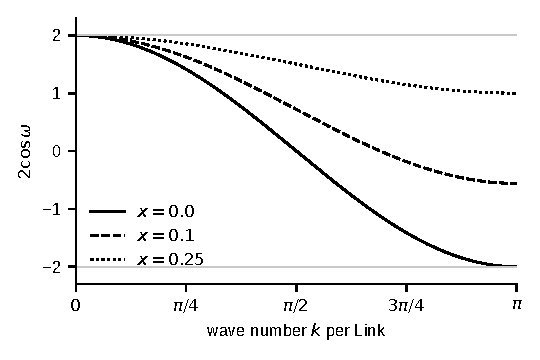
\includegraphics[width=0.62\linewidth]{figures/band.pdf}\caption{\label{fig:band}Light's band at a content $x = L / \Gamma$ read into the paces (\claimmark{derived}, Eq.~\eqref{eq:bandpace} at $\num = \den$): the doubled cosine of the rotation along one axis against the wave number, $2\cos\omega = 2 - 2(1 - 2x)^2(1 - \cos k)$, at $x = 0$, $0.1$ and $0.25$. The band's bottom rises with the content, its top stays at $2$; at the horizon $x = 1/2$ the band closes to a point. The slope at $k = 0$ is light's speed, $(1 - 2x) / \sqrt 3$ Links per interval. Drawn from the definitions; no run.}\end{figure}

\paragraph{The lattice constants.} The six Ports' own, exact and no number of nature: the massless row's rest around one static source of $s$ quanta per interval at the divisor $1$, by the start's iteration on an open box with its faces' constant image removed, is $3\,G(r)\,s$ with $3\,G(0) = 0.7582$ at the Node and $0.2582$, $0.1286$, $0.0826$, $0.0608$ and $0.0483$ at $1$ to $5$ Links, toward $3 / (4\pi) = 0.2387$ far away (\claimmark{computed}); of which $0.76\,s$ at the Node and $0.24\,s / r$ beyond are the continuum's; and light's $1 / \sqrt 3$ \cite[the lattice constants]{algebra}.

\subsection{The conserved form}\label{sec:form}

The read matrix $2\,\num\,p_i^2$ is not symmetric where the paces differ, so the form carries the weight $1 / p_i^2$ on the Node terms and the plain current on the Links:
\begin{equation}\label{eq:form}
E = \sum_i \frac{w\,(\mathrm{now}_i^2 + \mathrm{before}_i^2) - S_i\,\mathrm{now}_i\,\mathrm{before}_i}{p_i^2} - 2\,\num\sum_i \mathrm{now}_i\,S_6(\mathrm{before})_i .
\end{equation}

\begin{theorem}[the conserved form]\label{th:form}
At constant paces $E$ is exact under the line without the rounding; with the rounding each Node's remainder adds at most one unit of the level per interval to the walk of $E$. Its Link term, the plain current $\num\,(\mathrm{now}_i\,\mathrm{before}_j - \mathrm{before}_i\,\mathrm{now}_j)$ through the Link $ij$, is the current of Rule3's own conservation law.
\end{theorem}

\begin{proof}
Without the rounding the line is $\mathbf a_{\mathrm{next}} + \mathbf a_{\mathrm{before}} = \bM\,\mathbf a_{\mathrm{now}}$ with $\bM$ the matrix whose diagonal is $S_i / w$ and whose entries on the six Links are $R / w$. Let $\bD$ be the diagonal matrix of the weights $1 / p_i^2$; then $\bD\bM$ is symmetric, since $R_a = 2\,\num\,p_a^2$ at the reading Node and the weight $1 / p_i^2$ cancels it on both sides of every Link. For a symmetric $\bK = \bD\bM$ the quantity $Q(\mathbf x, \mathbf y) = \mathbf x \cdot \bD\mathbf x + \mathbf y \cdot \bD\mathbf y - \mathbf x \cdot \bK\mathbf y$ satisfies $Q(\mathbf a_{\mathrm{next}}, \mathbf a_{\mathrm{now}}) = Q(\mathbf a_{\mathrm{now}}, \mathbf a_{\mathrm{before}})$: with $\mathbf a_{\mathrm{next}} = \bM\mathbf a_{\mathrm{now}} - \mathbf a_{\mathrm{before}}$, $\mathbf a_{\mathrm{next}} \cdot \bD\mathbf a_{\mathrm{next}} - \mathbf a_{\mathrm{next}} \cdot \bK\mathbf a_{\mathrm{now}} = \mathbf a_{\mathrm{before}} \cdot \bD\mathbf a_{\mathrm{before}} - \mathbf a_{\mathrm{before}} \cdot \bD\bM\mathbf a_{\mathrm{now}}$, which is the other side. Multiplied by $w$ this is $E$ up to the Link term's sign convention \cite[the conserved form]{algebra}.
\end{proof}

$E$ is a GameBoard reading. It changes by the work term where the paces move: the total form $D = |\mathbf a_{\mathrm{now}}|^2 - \langle \mathbf a_{\mathrm{next}}, \mathbf a_{\mathrm{before}}\rangle$ of a record under paces that change in time obeys exactly $D(t + 1) - D(t) = \langle \mathbf a_{\mathrm{next}}, (\bM(t) - \bM(t + 1))\,\mathbf a_{\mathrm{now}}\rangle$ (\claimmark{theorem}, by substitution), $0$ at fixed paces and negative where a well deepens; the record's share of quanta, read from the same form in the vacuum's coefficients, is kept meanwhile: the mass defect is the form's fall at a kept count (Section~\ref{sec:bodies}) \cite[the mass defect is the form's fall at a kept count]{algebra}.

\subsection{The tension: the momentum's flux is the wave's own stress}\label{sec:tension}

The momentum density along the axis $a$ at the Node $i$ is the current per axis, $P_a(i) = (F_{i,i+a} - F_{i,i-a}) / \num$, and Rule3's line gives exactly, at constant paces (\claimmark{theorem}),
\begin{equation}\label{eq:momentum}
\begin{aligned}
w\,[P_a(t + 1) - P_a(t)] &= \sum_b R_b\,[G_{ab}(i - b) - G_{ab}(i)],\\
G_{ab}(i) &= \mathrm{now}_i\,(\mathrm{now}_{i+a+b} - \mathrm{now}_{i-a+b}) - \mathrm{now}_{i+b}\,(\mathrm{now}_{i+a} - \mathrm{now}_{i-a}),
\end{aligned}
\end{equation}
$G_{ab}(i)$ the stress booking on the $b$-Link $(i, i + b)$ at one time, the levels now alone; the proof substitutes $w\,\mathrm{now}' = \sum_b R_b (\mathrm{now}_{i+b} + \mathrm{now}_{i-b}) + S\,\mathrm{now}_i - w\,\mathrm{before}_i$ into $w\,P_a(t + 1)$: the $S$ term cancels, the $w$ term is $w\,P_a(t)$, and the $R$ term is the difference of the fluxes. So the flux of the $a$-momentum across the $b$-Link is $-(R_b / w)\,G_{ab}$, the second booking of the conserved form (its Link term shifted by one Link), and the tension on the axis $a$ at the Node, the part Rule3 reads into the Link's pace and the source of the held row's axis part $aa$, is the momentum's flux, the mean over the Node's two $a$-Links,
\begin{equation}\label{eq:tension}
\begin{aligned}
T_{aa}(i) &= -\num\,\bigl(G_{aa}(i) + G_{aa}(i - a)\bigr) \ddiv 2,\\
G_{aa}(i) &= \mathrm{now}_i\,(\mathrm{now}_{i+2a} - \mathrm{now}_i) - \mathrm{now}_{i+a}\,(\mathrm{now}_{i+a} - \mathrm{now}_{i-a}),
\end{aligned}
\end{equation}
the neighbour's own difference brought through the Port and no other shift: the tension on a Link is the booking of its two ends' own readings, a level and a difference each, and a Node sources its tensions with half of each of its Links, so the line is local as $F$ is. With the rounding the identity holds up to the remainders' term, $-r'_i\,\Delta_a\mathrm{now}_i + \mathrm{now}_i\,(r'_{i+a} - r'_{i-a})$, exactly. It is read and never written, quadratic in the amplitude as the form is: a plane wave of amplitude $b$ at the wave number $k$ has $G_{ab} = -2\,b^2 \sin k_a \sin k_b$ exactly, so the flux along the wave is positive, as a wave's pressure is; a uniform record gives $0$; a standing body's tail carries a tension that does not vanish in the mean; for a packet of count $c$ and velocity $\mathbf v$ it is $c\,v_a v_b$ within the rounding, the dust's stress with no count in any divisor and nothing undefined at a count $0$. With the sign as written a wave's stress deepens the content around it: light gravitates by its pressure too. The off-diagonal parts and the vector part, which Rule3 never reads, are not written \cite[the tension; the final unification]{algebra}\cite[the tensor part is the wave's own stress]{decisions}.

\subsection{The one write}\label{sec:write}

Every write into a family's level on the GameBoard is one act, the third line of Eq.~\eqref{eq:law}: $(w\,q(\text{Node}) + r) \ddiv E$ at a Node each interval, the division act with the remainder $r$ carried at that Node; $q$ the writer's own quantity there (a family of quanta's well $D_i \ddiv T$, its Wronskian's quanta, or its tension $T_{aa}$), $w$ the one weight of the pair of families (whoever reads with $w$ sources with $w$), $E$ the written row's divisor ($E_s$; $E_s \Wc$ for a tension, one act per axis). The hold, the well and the start are its instances; no number is the act's own. Generic (the rows' keys), vector (one carried division), local (the Node) \cite[the primitives]{algebra}\cite[the one algebra]{decisions}. The form $D_i = \mathrm{now}_i^2 - \mathrm{next}_i\,\mathrm{before}_i$ of a record at a Node is its well's source: for a standing record it is $B^2\sin^2\omega_b$ at every interval, $B$ its peak \cite[the gate reads the form at any phase]{algebra}.

\subsection{The interval and its inverse}\label{sec:interval}

The engine steps every family from the state at the interval's start to the state at its end; every read is of the start's values, one Link per interval and nothing in zero time. Before the first interval the whole initial state is checked once against the guard; then the interval has four acts, in order: (i) the signed read, every family's paces from the held families' levels at the start; (ii) Rule3 on every record, each family of quanta's two level pairs by its pair and its paces, each holder of the content's parts at its own pair at the pace $1$, and the bookings of its form and its Wronskian's quanta as the step left them; (iii) the detectors' reading, the net current through each declared region's front boundary, and the tension on each axis booked beside it; (iv) the hold, each held family's time part gaining its source over its divisor and its tensions the sources' momentum fluxes; light is born here, by the write of a rotating body's varying Wronskian into the sign holder's record \cite[the interval]{algebra}\cite[the interval]{engine}.

Backward, the acts run by Rule3's direction $-1$: a held row's hold back once every family that sources it is booked back, a family of quanta booked back once its own hold is off, so the holder of the sign goes before the rows it sources; every interval returns bit for bit, since every level a family read at the interval's start is one the state after the interval still holds, and only the lay of the first act is not taken back. The back-in-time gate is the whole run: $N$ intervals forward and $N$ back, every array of every family compared bit for bit at every interval on the way back, \textsc{match} or \textsc{miss} naming the first interval and the first Node that differ; a look is not run before it says \textsc{match} on the look's own world (\claimmark{theorem} by construction, from Theorem~\ref{th:direction}, the hold's carried division being its own inverse once every family that sources it is booked back). On the two slits' three worlds of Section~\ref{sec:slits} it says \textsc{match} over their $130$ intervals, on Bell's first world over $130$ and on the two speeds' worlds over $120$ \cite[the interval; what is open, item 21]{algebra}\cite[the board goes back in time, as a gate]{decisions}.

\subsection{The three channels}\label{sec:channels}

One family acts on another in three ways and no fourth (Fig.~\ref{fig:channels}): \emph{the read}, at (i), a held row's level times the read's weight into the reader's paces, the clock once and the Link twice, multiplicative, the whole of gravity, of binding and of the charge's pull; \emph{the write}, at (iv), the writer's own quantity through the one weight and the written row's divisor into the held row's level, additive, the source of every field and the birth of light; and \emph{the click}, at (iii), a declared detector's reading of the current through its boundary, the measurement alone, which writes nothing on the board. No product of two levels is written anywhere. No bilinear coupling between families is in the law: the world of clicks (bodies, detectors, the counts) and the world of Nodes (the records) run as one loop and touch only at the click and at a body's Nodes; a record sources the families its own family reads, so every pair of families that read each other is reciprocal, action and reaction one key \cite[the coupling is the click alone; light is born by the write]{decisions}.

\begin{figure}[!tb]\centering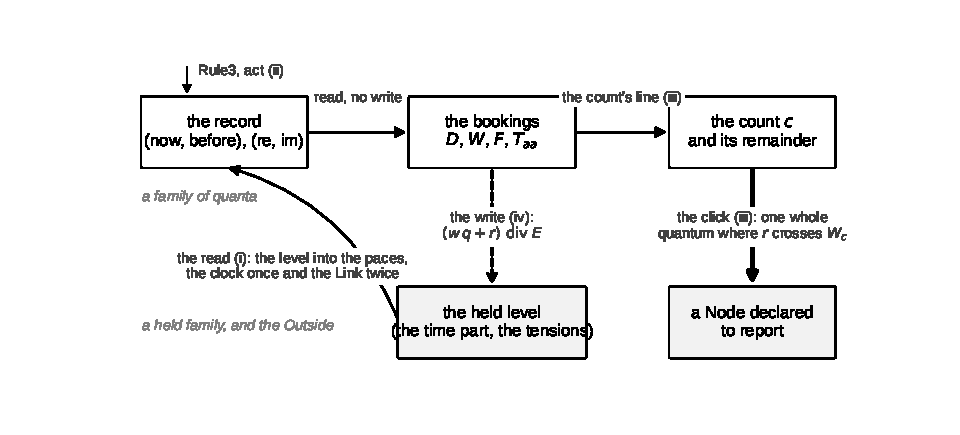
\includegraphics[width=0.78\linewidth]{figures/channels.pdf}\caption{\label{fig:channels}The three channels through which a family acts on another, drawn from the interval's four acts (Section~\ref{sec:interval}). A family of quanta steps its record by Rule3 and books its form and its current; a held family carries a level. The read (i) takes the held level into the record's paces; the write (iv) takes the record's form, its Wronskian's quanta and its tension into the held level over the row's divisor; the click (iii) is a declared region's reading of the current through its boundary, summed over the passage, one quantum per wall $\Wc$ of inflow, credited by the instrument. Every arrow is one line of Eq.~\eqref{eq:law}. Drawn from the definitions; no run.}\end{figure}

\section{The click}\label{sec:click}

The click is a detector's reading of the record and no act of the board: a declared region of Nodes sees the record's current through its boundary, the quantum's action measures it, and the instrument credits each quantum to one detector. This section states the three bookings the law reads from a record, the detector as a declared instrument with its credit, the lines that left the law, the no-wave rule, the sign, the birth of light, what the click ends (nothing), the price of locality and the postulates \cite[the click; the reading]{algebra}.

\subsection{The three bookings}\label{sec:booking}

A booking is a reading of a bilinear form of the levels with declared coefficients; it writes nothing on the board (Theorem~\ref{th:acts}). The law reads three, the third line of Eq.~\eqref{eq:law}. The form of a record at a Node, $D_i = \mathrm{now}_i^2 - \mathrm{next}_i\,\mathrm{before}_i$, $B^2\sin^2\omega_b$ at every interval for a standing record of peak $B$, whose quotient over $T$ is the record's quanta as the fields' source, the well (Section~\ref{sec:write}). The Wronskian $W_i$ of the record's two level pairs, the sign (Section~\ref{sec:sign}). And the current of a record into the Node $i$ from its neighbour $j$ through their Link over an interval, $F_{ij} = \num\,(\mathrm{now}_i\,\mathrm{before}_j - \mathrm{before}_i\,\mathrm{now}_j)$, positive inward: a record of wave number $k$ travelling from $i$ to $j$ has $F_{ij} = -2\,\num\,|\psi|^2\sin\omega\sin k$, below $0$. It is antisymmetric, $F_{ji} = -F_{ij}$, and it is the Link term of the conserved form (Theorem~\ref{th:form}), the current of Rule3's own conservation law; the lattice's continuity holds for it exactly, the change of a Node's form over one interval being the net current through its six Links at the levels the step started from (the advisor's check to $10^{-15}$), so the net current through a closed surface over a passage is the form that entered it \cite[the booking; the conserved form]{algebra}. A static record has $\mathrm{now} = \mathrm{next} = \mathrm{before}$, so its form is $0$ and its current $0$ at every Link: a static field carries no quanta and no detector sees it, by the arithmetic and not by a clause \cite[the count's line runs on every record]{decisions}.

\subsection{The detector is a declared instrument}\label{sec:detector}

\begin{assumption}[the detector's declaration]\label{as:detector}
A detector is a region of Nodes declared in the file, never one Node, at least half the wavelength of the family it reports across the beam ($q / p$ Links for the wave $[p, q]$, $4$ at $\lambda = 8$) and one layer deep along it; a narrower region is refused by name at load. It is opaque: backed by a receding face or by the wall's own face, so that what enters it leaves the declared board and never returns, with no act at its Nodes and no log. It sees the net current through its front boundary, the Ports leading in from the declared board, summed in integers over the passage; one wall $\Wc = 3\,\den\,T$ of that inflow is one quantum, so a screen saw $N$ quanta where its regions' inflows sum to $N\,\Wc$. The credit: one click per quantum to one detector, drawn by the shares of the regions' inflows, the host's reading over every declared detector of the world, one credit per quantum and never two; a click is reported with the region, the family and the Ports crossed, and never a Node. The credit is the one non-local place of the description and no line of the law.
\end{assumption}

The owner's words of 2026-09-30 and the advisor's definitions \cite[the count's line; no click names a Node; what produces a click is not known]{algebra}\cite[no click names a Node; what produces a click is not known; the two experiments' details under the new laws]{decisions}. Why a region: a quantum with a direction has no Node, a record confined to one Node being every wave number at once, $\Delta x\,\Delta k \ge 1 / 2$ on the lattice as in nature, and the finest structure the amplitudes of a family carry is half its wavelength, two split events of one wave number meeting at the smallest spacing that keeps their signs apart; so no click names a position finer than the region, and every per-Node number of a run is a GameBoard reading. Why the net front inflow: adjacent regions share transverse Links, and a density that entered one region and moved to the next inside the layer is credited where it entered, the click's place; the sum over the regions is the screen's total exactly, by the continuity, and the laid quanta less that total is the part that left elsewhere, reported beside it. Why opaque: a region whose back faces declared Nodes passes the density on and its net inflow reads nothing, and a layer written to $0$ reads to its neighbours as an open face and reflects; backed by a receding face the region removes from the declared board exactly what a cancelling write would, with no echo and no act, the two the same state within the declared board. What the law gives and what the instrument declares, precisely: what produces a click on the board is known and deterministic, the current of the amplitudes through the region's boundary, an emitter's events bringing inflow wherever they reach a detector, a bound body at its edge when it has a current (moving, breathing or in a well's gradient), a standing symmetric body cold; what is not known is which of the possibilities becomes the measured click: when one possibility is spread over several detectors the board gives the shares and no line of the law gives, exactly, which detector fires, and the instrument draws. Exclusivity (one click per quantum, never two) and Born's rule (the credit's chance the intensity's share) are therefore the instrument's declaration and no finding of the law, for nature or against it; nature's detector efficiency and dead time are declarations of the same kind \cite[what produces a click is not known]{algebra}. A detector is no body: no read by a sense and no resonance; the source of the two experiments is a laid message, the wall a declared face, and a body is the law's name for a standing record, matter, whose algebra of absorption stands parked with the pixel (Section~\ref{sec:nothing}) \cite[the click ends nothing]{decisions}.

\subsection{The lines that left}\label{sec:left}

Until the owner's word of 2026-10-01 the law carried two more lines at every Node, and the paper's earlier drafts were written on them: the count's line, $\Wc\,c_{\mathrm{next}} + r' = \Wc\,c_{\mathrm{now}} + \sum_j F_{ij} + r$ with $0 \le r' < \Wc$, a count $c$ of quanta per family at every Node with a remainder, moved by the division of the current, a quantum moving whole where the remainder crossed the wall, laid once from the record's share, conserved exactly by a telescoping sum, with the hole $-1$ where a total went below $0$ and the click as that division at a detector's boundary Port; and the sense's line, the same division on the Wronskian's current, moving the sign. The owner's word, verbatim: ``the count's line and the sense's line are thrown out'' (\claimmark{assumption}, the decision; the documents follow it by the Boss's hand, and the paper states it as the owner gave it). What the two lines gave, the record gives alone: the well is the form over $T$, read from the record each interval; the sign is the Wronskian, read from the record; what a detector sees is the current through its boundary, read from the record; and a body's quanta are the share of its record, a reading. The count's conservation theorem, the remainder's origin, the lay of the counts, the holes and the line's own pair creation, the anti-body as a lay of $-1$ and the velocity row of the count's centroid leave with the lines; so does the engine's one-interval lead of the count against its record (the count's line read its currents at the levels the step produced, while the continuity holds at the levels the step started from), which the paper had reported as an open question and which no longer arises. What stays is what the documents' runs showed on the lines' way out, a GameBoard reading and no claim: the whole quanta the count's line carried across a screen's boundary agreed with the current the screen saw to the rounding's order, $267$ against $284$ on the two slits' bright world and $405{,}080$ against $406{,}020$ over Bell's $32$ runs, so the reading of Assumption~\ref{as:detector} is the one those lines read too. The algebra of the exclusivity, two lines of the same day that moved the quantum itself and gave one entry per quantum at the price of the bit-exact inverse of the quantum's place, stands in the law's document under its own name and not in the law \cite[the algebra of the exclusivity]{algebra}. The back-in-time gate reads the records, their remainders and the holds' carries, bit for bit.

\subsection{No waves on the event board}\label{sec:nowaves}

On the GameBoard there are events, which split by Rule3 (each Node's level to its six neighbours, every possibility at once), and amplitudes, the levels Rule3 produces at the Nodes (the sum of the split events there, the record); in our world there are clicks, the detectors' reports, and nothing else. What nature calls a wave is, on the board, an emitter's events that spread (a laid message is an emitter's events declared in the file; a breathing or moving body's write is an emitter's events) and a detector that measures them or not; between the two ends there are events and amplitudes and no wave. The two slits' packet of light is the emitter's events; the fringes are where split events meet with the same sign at the screen; interference is split events meeting with opposite signs. What is compared with nature is clicks with clicks; what stays on the board, the empty amplitudes, is not in our world and changes a click only where it meets another event that is realised, which the receding faces prevent (\claimmark{assumption}, the owner's word of 2026-09-30) \cite[no waves on the event board]{algebra}\cite[no waves on the event board]{decisions}.

\subsection{The sign is the rotation sense}\label{sec:sign}

A family of quanta carries its record as two level pairs, $(\mathrm{re}, \mathrm{im})$, two solutions of the same line stepped by one call of Rule3 with one set of coefficients, each with its own remainder; a held family's parts stay real. The charge density at a Node is the booking
\begin{equation}\label{eq:wronskian}
W_i = \mathrm{re}_{\mathrm{now}}\,\mathrm{im}_{\mathrm{before}} - \mathrm{im}_{\mathrm{now}}\,\mathrm{re}_{\mathrm{before}},
\end{equation}
the Wronskian of the two pairs, which Rule3 conserves exactly with the conserved form's weights $1 / p_i^2$ (\claimmark{theorem}, $\bD\bM$ symmetric), its local change the Link current $\num\,(\mathrm{im}_i\,\mathrm{re}_j - \mathrm{re}_i\,\mathrm{im}_j)$ at the levels the step started from, so the sign is carried by the record's own line and needs no line of its own. A real record ($\mathrm{im} = 0$) has $W = 0$, so light, the sign holder's own real record, is neutral; a rotating record has $W$ of either sign by its sense, $-A^2\sin\omega$ for $e^{+i\omega t}$ and $+A^2\sin\omega$ for $e^{-i\omega t}$. The reader's $q$ at a Node is the sign of its own sense there; the holder of the sign is sourced by the Wronskian's quanta, $(W_i + r) \ddiv T$ each interval, over its divisor; the coupling goes as the sign, never as $Q / M$, so an electron and a proton accelerate alike in one field \cite[the sign is the rotation sense]{algebra}.

\paragraph{The charge is the record's.} For a record $(\mathrm{re}, \mathrm{im}) = (A\cos\omega t, e A\sin\omega t)$ the booking is $W = -e A^2\sin\omega$: the charge is the record's size times the ellipticity $e$ of the rotation, a property of the record that Rule3 conserves (the two levels obey one linear line, so their ratio is carried, not written). A circular quantum ($e = 1$) has $|W| / D = 1 / \sin\omega$; a nearly real cloud of $1{,}836$ quanta with $e = 1 / 1{,}836$ has the charge of one circular quantum; a body is one mode with one sense and one ellipticity at all its Nodes. What it costs, an input where nature has a measured number and no click row yet: nothing in the law quantises $e$, so a body's charge is continuous, and $|q_p| = |q_e|$, nature's to $10^{-21}$, is an input and not derived; the line that would derive it is a hypothesis under its own name, \emph{the second level's amplitude is a count of its own} (Section~\ref{sec:open}) \cite[the sign is the rotation sense; the hypotheses under their own names]{algebra}.

\subsection{Light is born by the write}\label{sec:light}

Light is the sign holder's own record: the holder of the sign is one record whose time part is its real level pair, stepped by Rule3 at the paces of its reads (the content, so light is bent) and written by the hold from the Wronskian's quanta of the families that read it by sign. A static rotating body writes a static level (its well in the sign holder, Coulomb's) and radiates nothing; a breathing or moving body writes a varying source at its Nodes, the row carries it away at one Link per interval in the vacuum, and those spreading events are the light (\claimmark{derived}). Its quanta need no lay and no conversion: a detector reads the light's current through its boundary like every record's, in quanta of $\Wc$; the held rows' travelling events, the quanta of what nature calls a gravitational wave, the binding holder's and the polarisation's, enter a detector the same way, the law's prediction and no declaration, and a static field is seen by no detector. A body's quanta that leave it stay its family, messages of matter; no quantum changes family at a crossing, no ledger of bodies stands beside the Nodes, and a body's Nodes are where its record stands bound about its declared Nodes. A body reads the sign holder by its own sense at its own Nodes, so a breathing body reads the light it writes and its pace answers, the radiation reaction, in the same loop \cite[light is born by the write]{algebra}\cite[light is born by the write; the count's line runs on every record]{decisions}.

\subsection{The click ends nothing}\label{sec:nothing}

\begin{assumption}[the click ends nothing]\label{as:nothing}
The click is a detector's reading, local to its boundary; the record goes on after it and nothing ends anywhere. What a detector absorbed leaves the declared board through the face that backs it and no echo goes back; the other possibilities go on splitting and leave through the receding faces, events that were not realised, in no click. The ending of a record at a click by the detector, a Node that takes the quantum into its own count, is decided against and is no hypothesis of the law.
\end{assumption}

The owner's decision of 2026-09-30 \cite[the click ends nothing]{decisions}, the law's claim and not a deficiency: perhaps nature is local. No signalling holds trivially, since nothing at one detector changes the amplitudes at another; the Outside reads the clicks alone. Absorption by a body, the algebra of matter, is a body's own act and no act of the law: a family of quanta reads the sign holder's level by its sense into its paces, a drive at the light's frequency, resonant where it meets the body's rotation (the parametric line, at twice the rotation), and the body's write answers, the driven body writing light of its own that cancels the incoming events behind it; a light quantum never becomes a matter quantum. It stands parked with the pixel, computed with the read alone in the documents' absorption look, row (y), a look of the documents and not an experiment of this paper; the detector of the two experiments is the declared instrument and no body (\claimmark{assumption}) \cite[the click ends nothing; the rows against nature, (y)]{algebra}.

\subsection{The price of locality}\label{sec:price}

The law's word, decided, read against nature's clicks alone \cite[what is open, item 4; the rows against nature, (g) and (h)]{algebra}:

\begin{enumerate}[leftmargin=1.6em]
\item[(i)] \emph{Exclusivity and Born, declared.} A quantum spread over several detectors is shares of the current at each; the law gives the shares and the instrument gives the click. The dilute world of the two slits, under one quantum per Node everywhere, rises click by click as Born by the declaration (Section~\ref{sec:slits-result}), and the earlier finding of the paper's drafts, that the pattern from single clicks does not form on a cold board, is a finding no more, for nature or for the law; the two takers' quarter (two far detectors both rising on one quantum with the probability $f_1 f_2$ under the count's line as it stood) is no claim read by a run, the credit standing in its place.
\item[(ii)] \emph{The which-way.} An opaque detector in one gap absorbs that gap's events whether or not it is credited, is credited about half the quanta, and the screen sees the other gap alone, no fringes, one gap's envelope: in nature a fully absorbing which-way detector is the closed slit, and the row is the same (Section~\ref{sec:slits-result}); a which-way marker that does not absorb is not in the law.
\item[(iii)] \emph{Bell.} The pair is one laid record, a common cause, its phase a shared classical variable inside Bell's $\lambda$ with the detectors' remainders and their history; the detectors are never at one Node and there is no joint read. A local reading that counts every quantum gives $|S| \le 2$, and the run gives $2.000$ to three places by the signs on both sides, the triangle's identity. Nature's $E = \cos(\delta_A + \delta_B)$ and $S = 2.76$ are reached by one declared instrument, a two-port detector that credits by its contrast and counts nothing where the two ports' shares are nearly equal, at the efficiency $0.64$: the uncounted pairs are those near the contrast's zero, the sample depends on the hidden variable and the setting, and that is the detection loophole of the Bell tests, closed in nature in 2015 at efficiencies above $0.83$ with the violation still seen; there, and only there, the law and nature part (Section~\ref{sec:bell}) \cite[Bell by the detector's contrast, the two slits as designed]{decisions}.
\end{enumerate}

The two slits read (i) and (ii), Bell reads (iii), and their rows are the law's answer, not a line to add. The paper writes them as they stand.

\subsection{The postulates}\label{sec:postulates}

\begin{enumerate}[leftmargin=1.6em]
\item The world is Nodes and Events. Space is the GameBoard; an Event is a wall crossed by a remainder at a Node, a level stepped; a click is a detector's; nothing else happens.
\item A Node holds bounded local information: its NodeState, fixed in size, read from itself and its six neighbours; no read beyond them, no list that grows with the world, nothing of the past kept. A self-field estimated or subtracted from anything global is forbidden, whatever the size of its final answer.
\item Consistency is local and causal: an Event first changes its own Node and travels Link by Link, one Link per interval, each Node updating on receipt under the same rule; the one exception is the production of a click, the instrument's credit of one quantum to one detector by the shares over every declared detector, the one non-local place, not known and not derived; and no quantum changes family at a crossing.
\item The causal speed is one Link per interval, built in; every other speed is a rational, a count of Links over a count of intervals.
\item Every physical calculation is on bounded integers; there is no float, no root and no draw in the law; a Node keeps only the law's own numbers: each record's level pairs and their remainders, the held rows' parts and their carries, the family's pair and the Node clock from the content there.
\item A measurement is a detector's click: one quantum credited to the declared region by the shares of the current its boundary saw, reported with the region, the family and the Ports crossed and never a Node; what produces a click is not known and not claimed. Only a click is compared with nature or pinned as an expectation; displays and the host's readings read state and write nothing.
\item The Inside is the GameBoard, where no one measures, deterministic and bit-reversible; the Outside is the detectors and their clicks, realised events, the only thing claimed to represent nature.
\end{enumerate}
\cite[the postulates]{algebra}

\section{The families from the rule}\label{sec:families}

A family is a band of the one rule and not a declaration, and its row holds nothing the rule and the geometry fix: its pair $[\num, \den]$, $\cos\omega_0 = \num / \den$, and what it holds, the content or the sign, at a divisor. Every pair is written over the GameBoard's one denominator $\Gamma$, so the file holds the numerator $m$ alone, $\cos\omega_0 = m / \Gamma$, and the wall is $w = 6\,\Gamma^3$ for every family; a reduction to lowest terms is a reading and never the loader's act, so every family's remainder has the one resolution \cite[the families from the rule; the mass is one integer; the wall is one]{algebra}.

\subsection{The exact bands, and the third closed as absent}\label{sec:exact}

The line of one Node at rest, $\anext = 2\cos\omega_0\,\anow - \abefore$, is exact in integers only where $2\cos\omega_0$ is an integer, so the rule carries exactly three exact rotations, $2\cos\omega_0 = 1$, $0$ and $-1$, the periods $6$, $4$ and $3$, the pairs $[1, 2]$, $[0, 1]$ and $[-1, 2]$ (\claimmark{theorem}). A record on an exact band at rest at the vacuum's pace leaves no remainder in its rest rotation, so it never clicks and only turns: no remainder, no click. The exact bands are exact only in the vacuum: at a Node of pace $p_0$ the band's rest rotation is $2\cos\omega = 2 - 2(\den - \num)(p_0 / \Gamma)^2$, an integer at $p_0 = \Gamma$ alone, so a record on an exact band inside a well leaves a remainder and clicks like every family's \cite[the exact bands; the exact bands are exact only in the vacuum]{algebra}.

The third, $[-1, 2]$, is a band the rule allows and the universe does not use, the mirror of $[1, 2]$: one family on it holds no standing body (its read is negative, so its own well pushes its rest rotation up into the vacuum's band and the record leaks). The three colours are the three axes of a click's Ports, a detector's reading of the click's axis, no charge of the body and no force of their own; whiteness is their balance at rest. So the quarks are not in the law: the white body, the tube, the charges $2/3$ and $1/3$, the generations, up and down leave with the third, and the band $[0, 1]$ of the period $4$ is the same, a band allowed and unused \cite[the third and the colours, closed as absent]{algebra}\cite[the colours are the three axes]{decisions}.

\subsection{The rule's own universe}\label{sec:universe}

The universe is the one whose every number is the rule's: the pairs from the integers $1$, $2$ and $3$ of the three exact rotations and the three axes, every divisor $1$ but gravity's, and the free numbers named. Its rows, as the file \texttt{examples/events/rule.json} holds them and as the rule derives the rest from the two keys of a row, its pair and what it holds (\claimmark{derived}) \cite[the families from the rule; the rule's own universe]{algebra}\cite[the loader and the files]{engine}:

\begin{center}\small
\setlength{\tabcolsep}{4pt}\begin{tabular}{L{3.4cm}L{2.2cm}L{3.0cm}L{0.9cm}L{4.6cm}}
\toprule
Family, its rank & Pair & Holds, at the divisor & Parts & Its free number\\
\midrule
gravity, the time part and the three tensions & $[1, 1]$ ($[6000, 6000]$) & the content, $E_g$ ($1{,}000$ in the looks, $10^6$ in the light-only worlds) & $1 + 3$ & $E_g$, the hierarchy; its rest $c_{\mathrm{vac}}$, $0$ by nature's clicks\\
the binding holder, the strong force; its own events have the gap $\cos\omega = \num_b / \den_b$ & $[2400, 2401]$ & the content, $1$ & $1$ & the pair, its range $R = 20$ Links, tied to $\Gamma$ by the proton\\
the charge, whose record's events are light, born by the write & $[1, 1]$ & the sign, $1$ & $1$ & none\\
the bound charge (the polarisation), the exact band & $[1, 2]$ ($[3000, 6000]$) & the content, $1$ & $1$ & none; a field of under one Link's reach\\
matter, the scalar; a quantum that leaves a body a message of matter & $[m, \Gamma]$ ($[4000, 6000]$) & nothing & $1$ & $m$, the mass\\
\bottomrule
\end{tabular}
\end{center}

\noindent The universe's integers: the Node clock $\Gamma = 6{,}000$, a multiple of $6$ so that every pair is exact over it; the quantum's action $T = 2^{15}$; the integers' width $63$ bits, a bound and no physics; and the vacuum content, the massless row's rest, $0$ by nature's clicks (Section~\ref{sec:vacuum}). Every family of quanta reads every holder of the content at the weight $1$ and the holder of the sign by its own $q$, and sources what it reads at the same weight; matter reads gravity and the binding holder plainly, $x = (L_b + L_g) / \Gamma$, the bound charge, and the charge by its sign; light reads the same holders of the content and is bent by them. The three of Rule3 is the three axes; the three axes give the three tensions the massless row carries beside its time part, $1 + 3$, the parts Rule3 reads and no other; every other family is a scalar. So the files hold $\Gamma$, $T$, the matter pair's $m$, the binding holder's pair, gravity's $E_g$ and the vacuum content, every other divisor $1$, and nothing else of physics; $\Gamma$ and $T$ are units, as $c$ and $\hbar$ are in nature, and no line of Rule3 fixes $T$, the rule being linear and its form's scale free. The crack, named: a second massive scalar family, a second mass, the rule does not forbid, and nature's spectrum of masses is the open row under this line \cite[the final unification]{algebra}\cite[two units and the bounds; the standing goal]{decisions}.

Every row of the file is a record stepped by Rule3 at its pair and sourced by the hold's division act, the vacuum's row and every holder with a gap alike; no laid row, no fixed point computed outside Rule3 during the run and no act beside the six verbs and the division act remains in the law or the engine; the start's rest is the fixed point of the division act with its remainder, the state Rule3 holds static, computed once by the generator (\claimmark{assumption}, the owner's word) \cite[nothing that is not Rule3 remains]{decisions}.

\subsection{The reach of a held family is its pair}\label{sec:reach}

A held family's rest solves $\num\,\Delta^2 a - 6(\den - \num)\,a = -3\,\den\,\sigma$ (its line with the source once an interval, $\Delta^2$ the six-neighbour second difference), so outside a body its rest falls by $e^{-\kappa}$ per Link with $\cosh\kappa = 3\,\den / \num - 2$, the family's own band at zero rotation: the gap is the mass of the records and the inverse reach of the field, one number (\claimmark{derived}). $[1, 1]$ has no gap and its rest is Poisson's over the whole GameBoard; $[1, 2]$ has $\cosh\kappa = 4$ and falls by $0.127$ per Link, a contact well of $0.41$ Links' reach; and a pair with $\num$ just under $\den$ has $\kappa^2 = 6\,\den / \num - 6$ to the second order, a range $R = 1 / \kappa = \sqrt{\num / (6(\den - \num))}$ Links \cite[the well]{algebra}.

\subsection{The two rows: the binding holder and gravity under a divisor}\label{sec:tworows}

\begin{assumption}[the two rows, decided with the caveat]\label{as:tworows}
The well of a record, $D_i \ddiv T$, is laid into two holders. The binding holder, a family with a gapped pair $[\num_b, \den_b]$, $\num_b < \den_b$, at the divisor $1$, stepped by Rule3 at its pair as the vacuum's row is and started at its rest, which with the gap is a sum with a range, $R = \sqrt{\num_b / (6(\den_b - \num_b))}$ Links and $e^{-r / R} / r$ beyond it: it binds the bodies, it is the law's strong force; its own waves have the gap $\cos\omega = \num_b / \den_b$, a quantum with a mass whose Compton length is $R$, Yukawa's own line and no input. The massless holder $[1, 1]$ at the divisor $E_g$ declared by the file: gravity, long-ranged and weak by $E_g$. A family reads both levels into its pace at the weight $1$.
\end{assumption}

The first pair is $[2400, 2401]$, $R = 20$ Links, $m^2 = 0.0025$, the quantum's rest frequency $0.029$ per interval, the pair tied to $\Gamma$ by the proton: a cloud of $1{,}836$ quanta is bound under $R = 20$ and not under $R = 10$ or $15$ (Section~\ref{sec:branches}). In the looks $E_g$ is the run's own number, large enough that gravity does not enter a body's binding ($1{,}000$ suffices at the pixel, $903 / 1{,}000$ under one level); nature's $E_g$ is about $3 \times 10^{42}$, $10^{36}$ times $1{,}836^2$, and the hierarchy is the file's one number, as $G$ is nature's. The reservation, in the owner's words, we may have been wrong: the line stands as a decision with a reservation and reopens on any of (i) the three tests, (ii) the bodies not standing under the screened sum, (iii) the charged cloud look reading electric over gravitational between two bodies as $E_g / 1{,}836^2$ and nature's other way, (iv) the finding of scale below, which this line does not touch and which may be the deeper error \cite[the two rows]{decisions}\cite[what is open, item 20]{algebra}.

\paragraph{The road not taken, kept as the law's word.} Under every divisor $1$ the force that binds a body and the force between bodies are one row, the well read at the weight $1$; the gravity between two quanta is then of order one against nature's $5.9 \times 10^{-39}$ for the proton, and the electric force between two protons, a charged cloud being a nearly real record with one unit of $W$ among $1{,}836$ quanta (Section~\ref{sec:sign}), is $1 / 1{,}836^2$ of the gravity between them, where nature's is $10^{36}$ times larger. That is the price of every divisor $1$ with its number, written as the law's word on its own universe, a computed number set beside nature's and no click \cite[the rows against nature, (v)]{algebra}. \emph{The reading of scale}, the same statement with no number: matter's rotation at rest, $\cos\omega_0 = 2 / 3$, fixes the electron's reduced Compton length in the lattice's units, light's speed over the rotation, $0.577 / 0.841 = 0.69$ Links; nature's proton is $1 / 400$ of that, $0.0015$ Links, while the law's cloud of $1{,}836$ quanta has the radius $2\Gamma / C$, at least $6.5$ Links at $\Gamma = 6{,}000$ and larger at every larger $\Gamma$: nature's proton is bound thousands of times smaller than the well binds anything, so the well row binds too strongly at a distance and too weakly up close to be both the proton's binding and gravity \cite[the rows against nature, (v) (2)]{algebra}.

\subsection{The vacuum content}\label{sec:vacuum}

\begin{assumption}[the vacuum content is $0$, a declaration fixed by nature's clicks]\label{as:vacuum}
The massless row rests at a declared level everywhere, the vacuum content, the key \texttt{rest} of the universe file, derived by no line of the law; nature's clicks fix it at $0$ in the file's integers at $\Gamma = 6{,}000$.
\end{assumption}

A constant is the massless row's own rest and its step keeps it ($\anext = S_6 \ddiv 3 - \abefore$ returns it); every reader's paces are $\Gamma - 2\,c_{\mathrm{vac}}$, the same physics at an effective $\Gamma$, so the law cannot tell $60$ from $0$ and only nature's clicks can. The clicks that fixed it, the first row of the calibration series (Section~\ref{sec:calibration}): light reads the vacuum content into its paces at the speed $(1 - 2x) / \sqrt 3$ while the massless row's own events step at $1 / \sqrt 3$, so the two arrive apart by $2xL\sqrt 3$ intervals over $L$ Links, and on the engine, as a look, light at no vacuum content arrived before light at the content $60$ by $21$ intervals at the centroids over $458$ Links against the blind $18$ from the two bands; nature's GW170817, the gravitational wave and the gamma-ray burst $1.7$ seconds apart after $1.3 \times 10^8$ years, bounds $|\delta c / c|$ below $10^{-15}$, so $c_{\mathrm{vac}} / \Gamma$ is below $10^{-15}$ and the file's integer is $0$: the law's cosmological constant is $0$ to every measurement's precision, the first number of the series entered as clicks. At the rest $0$ light reads only the bodies' wells and the field is non-negative wherever a well stands. The finding that gave the file a rest of $60$ for a day (a holder with a gap sourced by a changing well rings with its own travelling events, the law's mesons, whose troughs below $0$ far from the body light refuses, rightly, a real runaway of Rule3, Section~\ref{sec:paces}) stands as the reason for light's refusal below $0$ and not for a rest above it; the light-only worlds of Section~\ref{sec:slits} ran at the file's rest $60$ of the time and their rows stand, since a fringe's spacing and a calibrated phase read no rest \cite[what is open, item 22]{algebra}\cite[the vacuum content is 0, a declaration fixed by nature's clicks]{decisions}.

\section{The bodies}\label{sec:bodies}

\subsection{What a body is}\label{sec:whatbody}

A body is its record over its Nodes and the quanta that record carries, and never one Node: every body is many Nodes, and nothing gathers it. Its count, the number of its quanta, is the share of its record read in the vacuum's coefficients, $e_i = 3\,\den\,(\mathrm{now}_i^2 + \mathrm{before}_i^2) - \num\,\mathrm{now}_i\,S_6(\mathrm{before})_i$ over the wall $\Wc$, summed over its Nodes, a reading and no state of the board (Section~\ref{sec:left}); its form $D_i \ddiv T$ enters Rule3 through the pace alone, $x = (L_b + L_g) / \Gamma$. The record of the body's family splits by the read and is bound by the wells its counts source: by the binding holder's screened sum with the range $R$, while gravity's $1 / r$ is weak by $E_g$ and enters no body's binding \cite[what a body is]{algebra}. No law is written for a body: the one rule is written for the Node, and a body is the support of a mode of that rule; every proposal is a row at a Node or it leaves or is derived. A body has no law of motion of its own: its record moves by Rule3 alone, the count follows by the count's line, the momentum is a reading of the record's current, and in a pace gradient its packet accelerates as the mode's top velocity times its redshift per level times the level's difference across it \cite[what a body is]{decisions}.

The four lines of the body (\claimmark{derived} from the line, with the decisions named): (a) \emph{the body is the fixed point of its binding row}: its form sources every held row its family sources, its record is the standing record Rule3 makes in those paces, its count the weighted share that record lays, and it stands where the sources return themselves; (b) \emph{the form sources the fields}: a held row's level is the rest the start solves from the bodies' forms at the row's divisor, then Rule3 steps it; (c) \emph{the quanta follow the record}: a body's quanta are its record's share, carried wherever its record's current carries it, the well $D_i \ddiv T$ each interval being the record's quanta as the fields' source; (d) \emph{the fall}, for a free packet and for a cloud, $a = \Delta\,|d\omega_b / dc|\,\nabla c$, $\Delta$ the band's curvature at $k = 0$ and $d\omega_b / dc$ from Rule3's coefficients at the body's pace and rotation; a compact pixel falls by its tail alone, slower, so this line does not hold there. The world file names the body's family, its Nodes with their counts and the quanta of other families it holds, and nothing else: no momentum, no spin, no emitter, no sign, no seed, no stop, no period; its two levels are the generator's mode file beside the world \cite[the four lines of the body]{algebra}.

\subsection{The functional and the dilation}\label{sec:stable}

Let a body of $M$ quanta have the record $\phi$ over its region, $\sum\phi_i^2 = 1$, its counts the form $c_i = M\phi_i^2$, and let every held row $r$ it sources be a hollow ($\sigma_r = +1$) or a hill ($\sigma_r = -1$) with the static kernel $\mathbf G_r$ of its line, $(\Delta^2 - \kappa_r^2)\,a = -3\,\den\,\sigma / \num$ ($\kappa = 0$ for the massless row), and the divisor $E_r$, so that the well at a Node is $\Phi_i = \sum_r \sigma_r (M / E_r) \sum_j G_{r,ij}\,\phi_j^2$. To first order in $\Phi / \Gamma$ the well line raises the one-Node rotation $2\cos\omega$ by $4g\Phi / \Gamma$, $g = (\den - \num) / \den$, and there the fixed point of the binding row is a critical point on the sphere of
\begin{equation}\label{eq:functional}
F[\phi] = \frac{\num}{3\,\den}\sum_{\text{Links}} (\phi_i - \phi_j)^2 - \frac{2g}{\Gamma}\sum_r \sigma_r\,\frac{M}{E_r}\sum_{ij}\phi_i^2\,G_{r,ij}\,\phi_j^2,
\end{equation}
the band's pressure less the wells' energy, each well counted once for the record being its own source (Hartree's form; \claimmark{theorem}: the record is the top mode of Rule3's symmetric form at the paces, $\bM(\Phi) = \bM_0 + (4g / \Gamma)\,\mathrm{diag}(\Phi)$ at first order, and $dF / d\phi = 2\lambda\phi$ on the sphere is the fixed point's own equation with $2\cos\omega_b = 2\cos\omega_0 - \lambda$). Let $\phi_R(x) = R^{-d / 2}\phi(x / R)$ be the body dilated, $d$ the GameBoard's dimension; the pressure is $K / R^2$ and each row's well energy $W_r / R^{s_r}$, $s_r$ the row's scaling power at the body's size: $s_r = d$ beyond the row's reach (a contact), $s_r = d - 2$ within the reach or for the massless row (Poisson's $3 / (4\pi r)$ in a box) \cite[the functional and the dilation]{algebra}.

\begin{theorem}[the stable body]\label{th:stable}
At a fixed point of the binding row of width $R$ the virial $2K = \sum_r \sigma_r s_r W_r$ holds, and the second variation of $F$ along the dilation is $R^2 F''(R) = \sum_r \sigma_r s_r (2 - s_r)\,W_r$. A body is stable only where this sum is positive; it is a minimum of $F$ where further the Hessian on the modes orthogonal to the dilation and the translations is positive.
\end{theorem}

\begin{proof}
$F(R) = K / R^2 - \sum_r \sigma_r W_r R^{-s_r}$; $F'(1) = 0$ is $-2K + \sum_r \sigma_r s_r W_r = 0$; $F''(1) = 6K - \sum_r \sigma_r s_r (s_r + 1) W_r = \sum_r \sigma_r (3s_r - s_r^2 - s_r)\,W_r$: Derrick's scaling, Pohozaev's identity on the GameBoard \cite[the functional and the dilation]{algebra}.
\end{proof}

The signs: $s(2 - s)$ is $+1$ at $s = 1$, $0$ at $s = 2$, $-3$ at $s = 3$: a hollow holds the body where its well falls slower than the pressure and breaks it where it falls faster, and a hill does the opposite. From them: (a) one hollow beyond its reach binds every mass on a chain, is flat along the dilation on a plane, and in a box has one critical point, a maximum along the dilation, a saddle for every mass: the body disperses beyond it and collapses within it; (b) a massless row holds the body: Poisson's well in a box has $s = 1$, $F = a / R^2 - c / R$ has the one critical point $R = 2a / c$, a minimum for every mass (Pekar's body), its width falling as $E_g / M$; beside it a hollow beyond its reach adds a barrier, $F = a / R^2 - b / R^3 - c / R$ on a Gaussian body, the critical points $R = (a \pm \sqrt{a^2 - 3bc}) / c$, the wide one the minimum and the narrow one the saddle, none where $3bc > a^2$, the collapse; the largest mass with a minimum is $M_{\max} = a\sqrt{E_b E_g} / \sqrt{3 b_1 c_1}$ (\claimmark{computed}, the script beside the paper: on the matter pair $[4000, 6000]$ with a binding row of reach $2.02$ Links at $\Gamma = 6{,}000$, $M_{\max} = 4{,}450\sqrt{E_b E_g}$); (c) the horizon ends a collapse: beyond first order the well line saturates and the Link's pace weakens the pressure, both vanishing together at the pace's floor, so the collapse ends where a Link's pace reaches $0$, a frozen cluster of horizon Nodes and no body of ordinary matter; (d) the hill, a hypothesis under its own name, \emph{the hill holds the body}, and (e) \emph{the cooling}, the hypothesis that a body above its minimum sheds its excess as quanta of its own family and radiates light while it breathes, a cold body being one that has finished shedding. What is missing for the theorem to close: the Hessian beyond the dilation for a set of rows, the functional beyond first order, and the finite GameBoard \cite[the functional and the dilation]{algebra}.

\paragraph{The surplus leaves; the mass defect.} At a Node of a body's record the local rotation is read from its three levels, $2\cos\omega_i = (\mathrm{next}_i + \mathrm{before}_i) / \mathrm{now}_i$, against the local band's top; at a fixed point every Node is bound, and a cloud not at its fixed point has a free part, the Nodes whose rotation lies in the band, which leaves at its band's group velocity by Rule3 as it stands, its quanta with it. The bound surplus does not leave by itself, since a bound mode is stationary and Rule3 reversible (\claimmark{computed}, the script beside the paper: a cloud twice too wide in a static well breathes about its minimum for $6{,}000$ intervals with no settling), so evaporation sheds the free part alone. The mass defect is the form's fall at a kept count (Section~\ref{sec:form}): a standing mode in a well deepening from $300$ to $600$ at $\Gamma = 6{,}000$ loses $4.0$ percent of its form with its count kept, so a body that binds is lighter in every field it sources by its binding and no lighter in quanta; gravity's source is the well and the count is the baryon number \cite[the surplus leaves; the mass defect is the form's fall at a kept count]{algebra}.

\subsection{The two branches: the cloud and the compact pixel}\label{sec:branches}

The binding row's fixed point has two branches at every count above the edge, and the body of nature is the wide one (\claimmark{derived} from the fixed point, computed by the advisor; the reading the owner's decision) \cite[the two branches]{algebra}\cite[the body of nature is the cloud]{decisions}.

\paragraph{The cloud, the body of nature.} The wide branch, the continuum's Pekar body: the count spread over many Nodes, the radius about $2\Gamma / C$ Links for a count $C$. Its three masses, the well it sources (the sum over its Nodes of $D_i \ddiv T$, gravity's source), the count it resists with (the inertia, the momentum reading $n = 3\,Q\,j_a \ddiv T$) and the weight it falls with (the momentum identity's force term under a content gradient), agree to the order $(C / \Gamma)^2$, and it falls as a free quantum falls. Along its branch on an open $41$-cube at $\Gamma = 6{,}000$, matter $[4000, 6000]$, $T = 2^{15}$, under the massless row alone (the tension left out as of the order $(C / \Gamma)^2$ for a wide body), in the advisor's unit, the vacuum's share, which for a cloud is the engine's weighted share to a percent \cite[the rows against nature, (u)]{algebra}:

\begin{center}\scriptsize\setlength{\tabcolsep}{4pt}
\begin{tabular}{rrrrrrrr}
\toprule
Total count & $2\cos\omega_b$ (top $1.3333$) & rms radius & Centre Node & Well / count & Inertia / count & Inertia / well & Fall / free\\
\midrule
4,000 & 1.3509 & 8.7 & 2.6 & 0.985 & 1.061 & 1.077 & 0.92\\
3,000 & 1.3437 & 10.3 & 1.0 & 0.991 & 1.037 & 1.047 & 0.95\\
2,000 & 1.3383 & 11.5 & 0.4 & 0.995 & 1.022 & 1.027 & 0.97\\
1,500 & 1.3359 & 12.0 & 0.3 & 0.996 & 1.016 & 1.020 & 0.98\\
\bottomrule
\end{tabular}
\end{center}

\noindent The two lighter clouds lean on the box's faces, so their true radii are larger and their numbers nearer $1$ than the table shows. So Galileo and E\"otv\"os hold in the law for wide bodies to $(C / \Gamma)^2$, the better the larger $\Gamma$ is against the body's count. In the integer engine a cloud is sparse: at $1{,}500$ in all there are $0.3$ quanta at the densest Node, so the lay writes a quantum at a few hundred Nodes and none elsewhere, and the record shared by ten thousand Nodes carries them.

\paragraph{The compact pixel, collapsed matter.} The narrow branch: one Node and its tail, a standing record above the top of its family's band in the wells its own form lays, its count the sum over its Nodes, at one Node near the horizon and over its tail below it; a cluster is pixels within tail reach that click at one another. Its three masses part by the binding, since the gradient reaches its quanta only through its tail, where its own well has taken most of the Link pace ($(1 - 2x_0)^2 = 0.14$ at $2{,}000$). Along the narrow branch under the massless row with the tension (the counts in the advisor's unit; the engine's count about three times them, $3.7$ at the Node and $3.1$ in all at $2{,}000$) \cite[the rows against nature, (u)]{algebra}:

\begin{center}\footnotesize\setlength{\tabcolsep}{4pt}
\begin{tabular}{lrrrrrr}
\toprule
Count at the Node & Total count & The well & Well / count & The inertia & Inertia / count & Fall / free\\
\midrule
1,650 (the edge) & 2,541 & 1,769 & 0.70 & 2,642 & 1.04 & \\
2,000 & 2,640 & 1,637 & 0.62 & 2,621 & 0.99 & 0.27\\
2,500 & 3,005 & 1,636 & 0.54 & & & \\
3,000 & 3,449 & 1,692 & 0.49 & 3,105 & 0.90 & 0.11\\
4,000 & 4,413 & 1,860 & 0.42 & & & \\
4,500 & 4,917 & 1,967 & 0.40 & 4,069 & 0.83 & 0.03\\
5,000 (near the horizon) & 5,440 & 2,114 & 0.39 & 4,517 & 0.83 & \\
\bottomrule
\end{tabular}
\end{center}

\noindent A free quantum of matter at rest has a well equal to its count (a plane wave at $k = 0$ carries per Node the count $b^2(1 - (\num / \den)\cos\omega_0) / T$ and the well $b^2\sin^2\omega_0 / T$, equal at $\cos\omega_0 = \num / \den$), and a compact pixel's well is under its count everywhere in the window, $0.70$ at the edge to $0.39$ at the horizon: the binding lightens, the more so the deeper. Its inertia lies near its count and not its well, and its fall is suppressed, none at the horizon: a compact body sources gravity with its well, resists with its count and falls with its tail, the three masses parting by the binding. The horizon is a horizon, the pixel at the horizon a collapsed body and no proton, and gravity through the pace is not a metric for a compact body: a metric moves a body and its binding together, here the gradient moves the record and leaves its wells to follow, and the record is sheltered in them. That is the law's word on collapsed matter and no finding against nature, since nature's bodies are wide (Fig.~\ref{fig:branches}). The well has a minimum along the branch, $1{,}636$ at about $3{,}000$ in all, so accretion pays all the way to the horizon, where it ends. Between the two branches stands the saddle, where the total count falls with the binding (the Vakhitov and Kolokolov reading, $dC / d\lambda < 0$ with $\lambda = 2\cos\omega_b$) \cite[the three masses of a body; the two branches]{algebra}.

\begin{figure}[!tb]\centering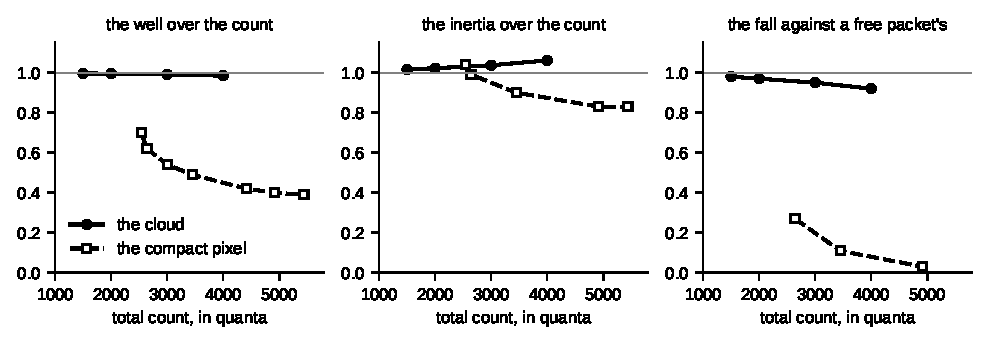
\includegraphics[width=0.9\linewidth]{figures/branches.pdf}\caption{\label{fig:branches}The three masses of a body along its two branches, from the documents' rows (\claimmark{derived} from the fixed point, a reading of the algebra and no click; the counts in the advisor's unit): the well over the count, the inertia over the count and the fall against a free packet's, for the cloud (the wide branch, filled marks) against its total count, and for the compact pixel (the narrow branch, open marks) against its total count. For the cloud the three go to one and the fall to a free quantum's the wider it is; for the compact pixel they part by the binding. Drawn from the rows of the law's document; no run.}\end{figure}

\paragraph{The electron and the proton.} The electron is one quantum of the matter family with the sense $-1$, a message and no pixel, stable by the integer (one quantum does not disperse into fractions), its charge the proton's exactly since the sense is a sign, the positron the same quantum in the sense $+1$; it needs no band of its own. The proton is a cloud of $1{,}836$ quanta, so $m_p / m_e = 1{,}836$ is the count's ratio directly, and it fixes no $\Gamma$: $\Gamma$ is free and large against $1{,}836$, as nature's Link is small against a proton. And $1{,}836$ is not derived: the law has one scale, $\Gamma$, and pure numbers of order one (the pair $2 / 3$, $\pi$, the lattice Green's function), so every count it derives is a fraction of $\Gamma$ or a small number, and a ratio of $1{,}836$ between two bodies needs $\Gamma$ or a large pure number the law lacks; the roads tried (the collapse count, about $0.5\,\Gamma$; the lightest cloud that binds at all, about $\sqrt{8.4\,\Gamma}$; their ratio; the coincidence $6\pi^5 = 1{,}836.1$) give none. So the proton's count is an input, an integer the world file declares as every body's count is, and the law fixes the electron's, one (\claimmark{assumption}, the owner's decision on the advisor's computation) \cite[the electron needs no band of its own; the rows against nature, (t)]{algebra}.

\paragraph{The second family's study, and the proton's size.} Two lines of Rule3 decide the road of a second, heavy family of matter before any fixed point (\claimmark{derived}, the advisor's study; its closing line waits on the owner's word). The fall of a free packet at rest in a content gradient $g$ depends on its pair's gap $\epsilon = (\den - \num) / \den$: $a / g = (1 - \epsilon) / (3(1 - \epsilon / 2))$, exact from the band, $0.2667$ at $[4000, 6000]$ and $1 / 3$ for a light pair, so the universality of free fall is one family's, and two families with different gaps would fall differently by up to a quarter where nature's materials fall alike to $10^{-13}$; the inertia of a family is $3\,\den\sin\omega_0 / \num$. And a body is never smaller than its quanta's Compton length, $0.577 / \omega_0$ Links, since a record localised to a size $R$ carries the band's kinetic shift about $1 / (6\omega_0 R^2)$ against a well of at most $\omega_0 / 2$ under the horizon; so the law's proton, a cloud of the electron's family, is at least the electron's Compton length across ($0.69$ Links at $\cos\omega_0 = 2 / 3$, the cloud's radius $2\Gamma / C$ beyond it), where nature's proton is $460$ times smaller. A heavy family with a Compton length of one Link gives a compact proton and breaks the fall's universality by the quarter; a light heavy family gives the fall and not the size; the two constraints together point to a proton of about three heavy quanta at a $\Gamma$ near $18$, which fails the fall: within Rule3 with the well as the binding there is no universe with nature's sizes and nature's fall, and the road closes. Under the rule that clicks are compared with clicks, the proton's radius and the electron's Compton length are both board numbers, so the statement is written only from a scattering look, short matter waves off a cloud onto a screen, whose blind row is that the cloud's pattern is as wide as the electron's Compton pattern or wider; the study stands as algebra until that look's rises are in. The study's record: the compact branch exists for a middling pair $[5000, 6000]$ too, tighter and with its fall more suppressed ($2\cos\omega_b = 1.7159$ at $2{,}000$ at the Node, $2{,}492$ in all, the fall $0.101$) \cite[the rows against nature, (v) (2); what is open, items 1 and 3]{algebra}.

\paragraph{The lightest body, and the pair tied to $\Gamma$.} Under the two rows a cloud stands only within the range $R$: under $[600, 601]$, $R = 10$, the cloud of $4{,}000$ stands ($2\cos\omega_b = 1.3367$, the rms radius $10.4$, its well $0.995$ and its inertia $1.02$ of its count, its fall $0.975$) while the clouds of $1{,}836$ and $1{,}000$ do not (their Poisson radii $12.2$ and $12.7$ Links, over the range); the binding holder holds no cloud lighter than about $1.5$ times $2\Gamma / R$, so there is a lightest body, the lightest cloud is the lightest baryon, the binding holder's own quanta are the mesons, and the electron is never a body. The cloud of $1{,}836$ is not bound under $R = 10$ nor under $R = 15$ ($[1350, 1351]$, $1.33320$, under the top by a hair) and is bound under $[2400, 2401]$, $R = 20$ ($2\cos\omega_b = 1.33394$, the rms radius $11.9$, its well $0.997$ and its inertia $1.011$ of its count, its fall $0.988$ of a free packet's), so the file's pair is $[2400, 2401]$ and $R$ is tied to $\Gamma$ by the proton, one number fewer in the file (\claimmark{computed}) \cite[the rows against nature, (w)]{algebra}\cite[the body of nature is the cloud]{decisions}.

\paragraph{The charged cloud, and the proton against the neutron.} The charge is the booking $W$, read into the pace at the weight $1$ as gravity's well is, so a cloud whose every quantum carried charge would have a hill of the sign holder equal to its gravity well and would not bind; the proton stands as a cloud of $1{,}836$ quanta with a total $W$ of one unit, its imaginary part a thousandth of its real one, one mode of one sense whose rotation is a thousandth elliptical. Derived beside it, a reading of the algebra set beside nature's number, no click and so no finding against nature: the charged cloud is bound a little less than the neutral one of the same count, by its own hill, so it is heavier by about $10^{-5}$ of its mass, where nature's neutron is the heavier, by $1.4 \times 10^{-3}$, opposite in sign and smaller \cite[the two branches; the rows against nature, (z)]{algebra}.

\subsection{The generator}\label{sec:generator}

The generator builds every world from zero, declares nothing and holds no float: the fixed point of the binding row by the law's own iteration, the mode under the wells its form lays and the wells from the mode, until the levels repeat; the two levels scaled together so that the weighted share the record lays carries the body's count; the held rows at their rest, the fixed point of the division act with its remainder, computed once before the first interval and never in it; a body laid with a sense carrying its second level pair, the record a quarter period on; a message laid by the file's keys alone, the wave under its envelope with its level one interval earlier, every cosine by Rule3's rotation act. The branch is selected by the start's width alone: from a wide start the iteration reaches the cloud, from a narrow start the compact pixel, two fixed points at one total, and the iteration goes to the one its start is nearer to, never across. The amplitude unit $A$ is derived from the integer width as the largest amplitude at which Rule3's total stays inside it, never written \cite[the generator]{algebra}\cite[the generator is Rule3]{decisions}.

\section{The forms of nature the line arrives at}\label{sec:forms}

Each form below is arrived at from the line before any run and is a prediction of the law, never a result; the form of nature beside it is on the comparison side and is never an input. The coefficients of Eq.~\eqref{eq:law} were written for the Node: a held level lowers the clock's pace once and the Link's pace once more, with no metric, no boost and no potential in them; what follows is what those coefficients do to a packet, read by the geometric optics of its band. $U_b = c_b / \Gamma$ is the potential at the point named, the clock's shift per level \cite[the rows against nature]{algebra}.

\begin{enumerate}[leftmargin=1.6em]
\item[(a)] \emph{The redshift} (\claimmark{derived}). Two clocks of one family at the levels $c_1$ and $c_2$ have their tick intervals in the ratio of the root of $(1 - 2U_1 + 2U_1^2) / (1 - 2U_2 + 2U_2^2)$, $1 - (U_1 - U_2)$ to first order, for a band whose rotation follows the clock's pace; the band's own slope: at the content $x$ a record of the pair $[\num, \den]$ at rest rotates at $2\cos\omega = 2 - 2((\den - \num) / \den)((1 - x)^2 + x^2)$, so for matter $[4000, 6000]$ $d\omega / \omega = -1.06\,x$ to first order and the gravitational redshift is the clock's share, $z = 1.06\,x$; light born by a breathing body in the well leaves with the body's rotation and keeps it in flight (a static content changes no frequency), so a far detector reads the emitter's slow clock. Beside it: Einstein's gravitational redshift.
\item[(b)] \emph{The bending} (\claimmark{computed}). At a Node of content $x$ light's index is $n = 1 / (1 - 2x)$, $n - 1 = 2x$, the Link's pace reading the content twice (Section~\ref{sec:paces}); far from a body its field is the massless row's rest, $L(r) = 3\sigma_{\mathrm{tot}} / (4\pi r)$ beyond a few Links, $\sigma_{\mathrm{tot}}$ the body's wells per interval, so $n - 1 = 3\sigma_{\mathrm{tot}} / (2\pi\Gamma r)$ and a beam past the body at the closest distance $b$ turns by $3\sigma_{\mathrm{tot}} / (\pi\Gamma b)$ radians, $4U_b$, the centroid at a receiver $L$ Links beyond shifted by $4U_b L$ toward the body. The ratio that is nature's: the bending is $2x$ and the redshift $1.06\,x$, so light is bent by $1.9$ times a matter clock's share (exactly $2$ against the clock's own share $x$, the $1.06$ the band's slope at $[4000, 6000]$), against nature's $2$, with no chosen number in it. By the geometric optics of the band from the coefficients themselves (the script beside the paper, both forms of the self coefficient): the deflection is $2.02$ times Newton's $2U_1 / b$ with the clock to the first order or the second, Einstein's $4U_1 / b$; with the Link's pace lowered once it would be $1.01$ times Newton's. Beside it: Einstein's $4GM / (c^2 b)$.
\item[(c)] \emph{The delay} (\claimmark{derived}). A round trip past the body is delayed by $4U_b$ times the path's length within the well's reach. Beside it: Shapiro's delay.
\item[(d)] \emph{The perihelion} (\claimmark{computed}). An orbiting emitter at the semi-axis $a$ and the eccentricity $e$ advances $6\pi U_p$ per orbit with $U_p$ the potential at $a(1 - e^2)$: by the same geometric optics the matter pair's periapsis advances $7\pi U_1 / (a(1 - e^2))$, $1.17$ times Einstein's, with the clock to the first order and $6\pi U_1 / (a(1 - e^2))$, $1.00$ times Einstein's, with the clock's second order, which is the line (Section~\ref{sec:paces}); the bending stays $4$ under both. Beside it: Einstein's $6\pi GM / (c^2 a(1 - e^2))$.
\item[(e)] \emph{The moving clock} (\claimmark{derived}). A body at the velocity $v = n / W$ (its phase $k$ per Link an exact pair of the file) has its tick lengthened by the dispersion of its own bound band: the tick's factor is $f = \Omega(k) / \omega_0$ with $\Omega(k) = \omega(k) - k\,\omega'(k)$ the rotation at the moving centre, the phase rate less $k$ times the group velocity, and $\omega(k) = \omega_0 + \Delta(1 - \cos k)$ the body's bound band, $\omega_0$ its rest rotation and $\Delta$ its packet's top velocity, both the generator's from the file's counts and pair, no key; to the second order $f = \sqrt{1 - v^2 / c_b^2}$ with $c_b^2 = \Delta\,\omega_0$, Lorentz's factor at the body's own light speed; read as the mean of the front and back click periods $P_v(1 \mp v / u)$ at two resting detectors, $u$ the light's group velocity, $P_{\mathrm{rest}} / P_v = f$. Beside it: Lorentz's factor, at the body's own light speed and not the lattice's, since no boost is among the $48$. Lorentz is arrived at as the symmetry of the clicks Outside, not as a symmetry of the lattice \cite[the click]{decisions}.
\item[(f)] \emph{The charge} (\claimmark{derived}). Like senses a hill, unlike a hollow; a reader of the sense $q$ reads $-q$ times the holder's level in its pace. The coupling goes as the sign: the read by sign enters the pace as $q$ times a level, never as $Q / M$, so an electron and a proton accelerate alike in one field, and the response in a gradient is the mode's own and not the coupling's. A current's read (the magnetic force, frame dragging) is a hypothesis under its own name and no line of the law. Beside it: Coulomb's force.
\item[(g)] \emph{De Broglie's relation} (\claimmark{derived}). A free record of a matter family travels only where its band holds its rotation, $\num / (3\,\den) \le \cos\omega_b \le \num / \den$; its wave number is the band's, $\cos\omega_b = (\num / (3\,\den))(2 + \cos k)$, its group velocity $v = (\num / (3\,\den))\sin k / \sin\omega_b$, and to the second order $k = \omega_b v / c_m^2$ with $c_m^2 = \omega_0 / (3\tan\omega_0)$, the family's own light speed. Beside it: $\lambda = h / p$ with the rest rotation as the mass.
\item[(h)] \emph{The fall} (\claimmark{derived}). In a pace gradient a free packet or a cloud accelerates at $a = \Delta\,|d\omega_0 / dc|\,(c_+ - c_-) / D$ toward the well, $c_+$ and $c_-$ the read level at its two faces $D$ Links apart, so bodies with the same $\Delta \times d\omega_0 / dc$ fall alike, and a cloud falls as a free quantum falls to $(C / \Gamma)^2$ (Section~\ref{sec:branches}); a compact pixel falls by its tail alone, slower; the universality is one family's, $a / g = (1 - \epsilon) / (3(1 - \epsilon / 2))$ with $\epsilon$ the pair's gap, and the law has one family of matter. Beside it: Galileo's fall and the equivalence principle, which hold in the law for the bodies of nature and not for collapsed matter.
\item[(i)] \emph{The pull and the orbit} (\claimmark{derived}). The massless row rests at Poisson's with the sources and at Laplace's outside a body, $c(r) = 3s / (4\pi r)$ falling to the faces' $0$, so the acceleration falls as $1 / r^2$ and a circular orbit's $v^2$ as $1 / r$; under the two rows a reader within $R$ reads the binding holder's screened field instead, and a row that reads $1 / r$ beyond $R$ takes $E_g = 1$ in its own world. Beside it: Newton's pull and Kepler's fall-off; a flat $v(r)$ would name a missing law.
\item[(j)] \emph{The medium} (\claimmark{derived}). Inside a body of pace $p$ light of wave number $k$ is slowed to $v_{\mathrm{in}} = (p / \Gamma)^2\sin k_{\mathrm{in}} / (3\sin\omega)$ with $1 - \cos k_{\mathrm{in}} = (\Gamma / p)^2(1 - \cos k)$, the index $v_g / v_{\mathrm{in}}$, and is reflected whole where $p < \Gamma\sin(k / 2)$; through a window moving at $w$ the wave number is matched at the moving face, $\omega - kw = \omega_{\mathrm{in}} - k_{\mathrm{in}} w$, and the speed inside is the band's group velocity at that $k_{\mathrm{in}}$. Beside it: the refractive index and the mirror; Fresnel's drag $w(1 - v_{\mathrm{in}}^2 / v_g^2)$ is nature's number beside it and not derived from it.
\item[(k)] \emph{The round trip and Sagnac} (\claimmark{derived}). A radiating body receding at $v$ from a mirror at rest reads its returned clicks every $P(u + v) / (u - v)$ intervals for a write every $P$, $u$ the group velocity at the wave number that solves $\Omega(k) + kv = \omega_b$; a radiating body moving at $v$ along a ring of $N$ Links reads its two arms $2Nv / (u^2 - v^2)$ apart, $4A\omega / u^2$ for the ring's area $A$ and angular speed $\omega$ to first order. Beside them: the two-way Doppler ratio and Sagnac's $4A\omega / c^2$, with $u$ in place of $c$.
\item[(l)] \emph{A free record keeps its wave number} (\claimmark{theorem}). Rule3 is translation-invariant, so a free record keeps its wave number and rotation exactly and a radiating body's period is read unchanged at every distance, the record's rows widening by the dispersion while its count does not move, the rounding's walk at most one unit of level per Node per interval. Beside it: Hubble's drift, which the law does not give from a fixed $\Gamma$; the law's own line for an expansion is the hypothesis \emph{Gamma is not constant} (Section~\ref{sec:open}).
\end{enumerate}

\paragraph{The numbers of one body.} For the $2{,}000$ pixel at $\Gamma = 6{,}000$ (\claimmark{computed}, the advisor's derivation): under Poisson's rest, the bending $0.26 / b$ radians, $3.0$ degrees at $b = 5$ Links and $1.5$ at $10$, a $\lambda = 8$ packet passing at $b = 6$ turning by $0.043$ radians, a transverse shift of $1.3$ Links over $30$ Links of path; a matter clock five Links from the pixel ($x = 0.013$) running $1.4$ percent slow against a far one. Under the two rows the massless row's field is over $E_g$ and a reader within $R$ reads the binding holder's screened field instead \cite[the rows against nature, (a) and (b)]{algebra}:

\begin{center}\footnotesize\setlength{\tabcolsep}{4pt}
\begin{tabular}{lrrrrrr}
\toprule
Distance from the pixel & \multicolumn{2}{c}{The field, in levels} & \multicolumn{2}{c}{The clock's share $z$} & \multicolumn{2}{c}{The bending at that impact parameter}\\
 & $[2400, 2401]$ & Poisson & $[2400, 2401]$ & Poisson & $[2400, 2401]$ & Poisson\\
\midrule
1 Link & 373 & 386 & & & & \\
2 Links & 189 & 205 & & & & \\
3 Links & 117 & 133 & & & 4.9 deg & 5.0 deg\\
5 Links & 62 & 79 & 1.09 \% & 1.4 \% & 2.8 deg & 3.0 deg\\
10 Links & 24 & 40 & & & 1.2 deg & 1.5 deg\\
\bottomrule
\end{tabular}
\end{center}

\noindent The bending stays $1.9$ times the clock's share under both; the lattice computation of it to three digits, a pixel of $2{,}000$ and a packet passing at five Links, the packet's deflection against the clock's share at the same Node, is the first proof-grade number the law offers (Section~\ref{sec:constants}): $2.00$ within the rounding is the direction confirmed, $1.9$ sharp a lattice correction to state \cite[the rows against nature, (b) and (v)]{algebra}.

\paragraph{How the forms are reached, not assumed.} Nothing above was put into the coefficients: no metric, no Lorentz transformation, no potential and no force. The one thing the law says is that a held level slows a Node's clock once and its Links twice, and that a record's rotation follows its band. The bending's $4$ and not $2$ is the Link's second factor; the perihelion's $6\pi$ and not $7\pi$ is the clock's second order, the composition of the slowing unit by unit; Lorentz's factor is the Legendre transform of a bound band read at its moving centre. Where the law's number differs from nature's form at the declared numbers, the difference is the law's own, read blind: the bending's $1.9$ against $2$ (the band's slope at the matter pair), Sagnac's $u$ against $c$, Fresnel's drag not derived.

\section{The two experiments: the two slits and Bell}\label{sec:slits}

The paper's experiments are two, the two slits and Bell, each a run of the engine against a blind row written first and no computation of the algebra; everything else the documents read on the board is a look, a GameBoard diagnostic, and not an experiment of this paper. Both are light-only worlds on the engine as it is, no body and no well in them, on the light-only universe file: the rule's own universe with the three holders' divisors at a million, so that light's own wells round to nothing (at the divisors of the rule's own file the two slits' packet laid a well of $752$ levels and its fringes' centre stood a third higher, a self-focusing of light that nature never shows at any intensity, kept in the documents as a finding by name and no row, and the bound on gravity's divisor it gives is in Section~\ref{sec:calibration}). Every number here is the law's document's, rows (g) and (h) of the rows against nature, and is cited so \cite[the rows against nature, (g) and (h)]{algebra}\cite[the two slits; Bell by the detector's contrast, the two slits as designed]{decisions}. The rule of the rows: an experiment checks only clicks; its operator, its tools, its conservation and its initial state are proved in the algebra and checked at load, never by a run; a run before its blind number is a first look and says so \cite[an experiment checks only clicks; algebra first]{decisions}.

\subsection{The two slits: the world}\label{sec:slits-world}

The emitter is a laid message, the emitter's events, a packet of the light family (the charge, the sign holder's own real record), no body: a wavelength of $8$ Links along $+x$, $k = \pi / 4$, $\cos\omega = 0.9024$, the period $14.1$ intervals, the group velocity $0.547$ Links per interval (light's speed at long wavelength is $1 / \sqrt 3$); its levels laid at the first act as $\mathrm{now}_i = b\,e_i\cos(k x_i)$ and $\mathrm{before}_i = b\,e_i\cos(k x_i + \omega)$, the record one interval earlier, with $b = 1{,}328$, about ten quanta per Node of the plane record, under a raised cosine along $x$ over $x = 4$ to $16$ centred at $x = 10$, flat across $y = 4$ to $44$ with edges of two Nodes, $1{,}797$ quanta laid; a real packet, neutral. The wall is not matter (a mirroring row of pixels is past the horizon by its summed fields) but the board's own face rule declared inside the board: the inner face at $x = 20$ with two gaps of three Nodes, $y = 17$ to $19$ and $29$ to $31$, the slits' centres $d = 12$ Links apart, a declaration of the file like the wraps and the detectors' regions, no number in the engine. The board is flat, $45 \times 48 \times 1$, the third axis folded, its $y$ faces open and its far $x$ face receding (the largest size $256$, $16$ layers of zeros per growth), so that the screen, the board's last column $x = 44$, $L = 24$ Links from the wall, is backed by the receding face itself and is opaque. The screen is twelve declared detectors, the regions of four rows of that column from the row $0$, the smallest region the law allows at $\lambda = 8$, each reporting what it saw. The run is $130$ intervals; the packet's centre reaches the wall at about interval $18$ and the screen at about $62$; the screen is read in the window of intervals $45$ to $120$. Three worlds: the bright packet as above; the dilute packet, $b = 420$, $85$ quanta laid, under one quantum per Node everywhere; and the which-way world, the lower gap closed by the wall's own face, the screen seeing the open gap alone (the design's pocket before the watched gap, backed by a receding zone at that gap, is not buildable with the receding face of an axis, a local receding face being an engine primitive still to be designed, so the closed gap gives the row and the watched gap's credit is read by continuity as the two screens' difference) \cite[the rows against nature, (g)]{algebra}.

The folded board is the experiment exactly and no special case: for a record uniform along $z$ the folded axis returns the Node itself through both $z$ Ports, so light's band on the flat board, $2\cos\omega = (2 / 3)(\cos k_x + \cos k_y + 1)$, is the three-dimensional band at $k_z = 0$, and the screened sums are the three-dimensional ones summed along $z$; a thick folded board with the same packet gives the same fringes with the counts multiplied by the thickness, and a thick open board is a second world (\claimmark{derived}) \cite[the rows against nature, (g)]{algebra}.

\subsection{The two slits: the blind row}\label{sec:slits-blind}

Written before the run, from the law's own lines (\claimmark{computed}): light's plain line on the very board in real arithmetic, the inflow through the screen's column over the window, $\sum F \ddiv \Wc$, per region. The formula: the far field's spacing $\lambda L / d = 8 \times 24 / 12 = 16$ Links; at $L = 2d$ the fringe is the near field's, the two gaps' path difference reaching half a wavelength $8.7$ Links from the centre and a whole one $22$ Links out, so the minima fall at the rows $15$ and $33$ and the outer maxima spread over the rows $0$ to $7$ and $40$ to $47$, under the three-Node gap's envelope. The numbers, \textsc{detector}: through the screen in all $273$ quanta ($15$ percent of the packet, the gaps' share less the wall's return), per region from the row $0$: $21$, $20$, $26$, $15$, $9$, $40$, $45$, $16$, $11$, $25$, $22$, $25$ (Table~\ref{tab:slits}); the clicks' row each detector's clicks $N$ times its share, the total exactly $N$ and the fluctuation per detector $\sqrt{N p (1 - p)}$ from the draw. For the dilute packet: $12.9$ quanta through the screen, the pattern by the declaration, $N$ times the shares. For the which-way world: the open gap's envelope over the regions, $3.7$, $4.9$, $6.5$, $8.7$, $11.3$, $14.1$, $16.5$, $17.6$, $16.9$, $14.8$, $12.0$, $9.3$, $136.5$ in all, no fringes \cite[the rows against nature, (g)]{algebra}.

\subsection{The two slits: the result}\label{sec:slits-result}

The run of 2026-09-30 on the light-only file: the back-in-time gate says \textsc{match} over $130$ intervals on each of the three worlds, and the three runs are \textsc{lawful}. \textsc{detector} (Table~\ref{tab:slits} and Fig.~\ref{fig:slits}): the bright world's screen saw $N = 284$ quanta over the window against the blind $273$, $1{,}513$ of the $1{,}797$ laid having left elsewhere, the wall's return through the source's face; the clicks credited by the shares, by the largest remainders, $21$, $20$, $27$, $16$, $10$, $42$, $48$, $15$, $12$, $27$, $22$, $24$ against the blind $21$, $20$, $26$, $15$, $9$, $40$, $45$, $16$, $11$, $25$, $22$, $25$, the deviation from the blind shares $0.18$ of the total, and one draw of the $284$ by the shares at the declared seed $14$, $20$, $32$, $16$, $12$, $37$, $48$, $13$, $14$, $31$, $23$, $24$, one quantum to one detector by the draw's construction; the centre fringe's two regions $90$ against $85$, the minima $16$ and $12$ against $15$ and $11$, the outer maxima in the edge regions where the near field puts them. Against nature: the fringes at the near field's places, from the local rule and the declared reading, clicks against clicks; every grain of nature's screen is a click and the fringes their histogram, every quantum credited to a region of this screen a click and the fringes their histogram. The dilute world: no region's inflow reached a wall at any interval, the packet riding under one quantum per Node everywhere, and the screen saw $N = 28$ over the run (the blind $12.9$; $57$ left elsewhere), credited $2$, $2$, $3$, $2$, $1$, $4$, $5$, $1$, $1$, $3$, $2$, $2$ against the blind $1.0$, $0.9$, $1.2$, $0.7$, $0.4$, $1.9$, $2.1$, $0.8$, $0.5$, $1.2$, $1.0$, $1.2$ and drawn $0$, $3$, $4$, $0$, $3$, $2$, $1$, $1$, $4$, $3$, $3$, $4$: the pattern by the declaration alone, as the design said, no finding either way. The which-way world: the screen saw $N = 142$ (the blind envelope $136.5$), credited $4$, $5$, $6$, $8$, $11$, $14$, $15$, $16$, $16$, $16$, $13$, $18$ against the envelope (the deviation $0.38$, the edge region $18$ against $9.3$), no fringes, one gap's envelope, the row nature gives with the slit closed; the watched gap's credit by continuity is the two screens' difference, $284 - 142 = 142$ quanta, $50$ percent \cite[the rows against nature, (g)]{algebra}.

\begin{table}[!tb]\centering\caption{\label{tab:slits}The two slits, \textsc{detector}: the quanta through each of the screen's twelve declared detectors over the window, the regions of four rows named by their first row, blind (written before the run) and the clicks credited by the shares, for the three worlds. From the law's document, row (g).}
\scriptsize\setlength{\tabcolsep}{4pt}
\begin{tabular}{l*{12}{r}r}
\toprule
The region's first row & 0 & 4 & 8 & 12 & 16 & 20 & 24 & 28 & 32 & 36 & 40 & 44 & In all\\
\midrule
bright, blind & 21 & 20 & 26 & 15 & 9 & 40 & 45 & 16 & 11 & 25 & 22 & 25 & 273\\
bright, the clicks credited & 21 & 20 & 27 & 16 & 10 & 42 & 48 & 15 & 12 & 27 & 22 & 24 & 284\\
bright, one draw by the shares & 14 & 20 & 32 & 16 & 12 & 37 & 48 & 13 & 14 & 31 & 23 & 24 & 284\\
\midrule
dilute, blind & 1.0 & 0.9 & 1.2 & 0.7 & 0.4 & 1.9 & 2.1 & 0.8 & 0.5 & 1.2 & 1.0 & 1.2 & 12.9\\
dilute, the clicks credited & 2 & 2 & 3 & 2 & 1 & 4 & 5 & 1 & 1 & 3 & 2 & 2 & 28\\
\midrule
the lower gap closed, blind (one gap's envelope) & 3.7 & 4.9 & 6.5 & 8.7 & 11.3 & 14.1 & 16.5 & 17.6 & 16.9 & 14.8 & 12.0 & 9.3 & 136.5\\
the lower gap closed, the clicks credited & 4 & 5 & 6 & 8 & 11 & 14 & 15 & 16 & 16 & 16 & 13 & 18 & 142\\
\bottomrule
\end{tabular}
\end{table}

\begin{figure}[!tb]\centering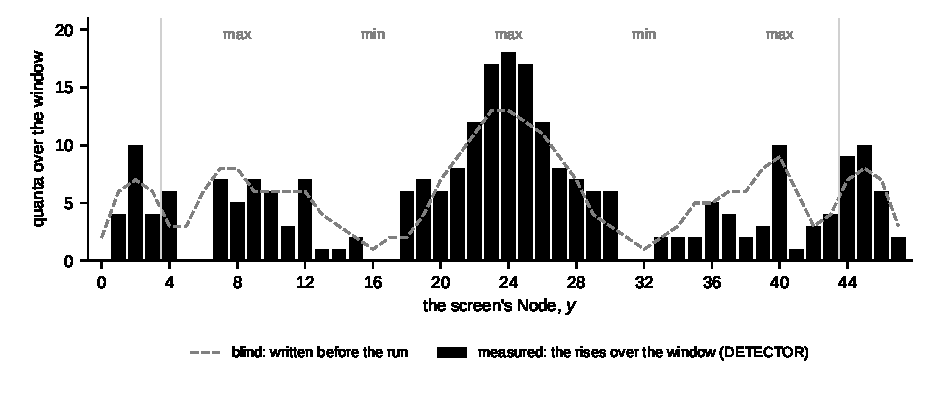
\includegraphics[width=0.98\linewidth]{figures/two_slits.pdf}\caption{\label{fig:slits}The two slits: the clicks credited to each of the screen's twelve declared detectors (the bars, \textsc{detector}, the measurement) beside the blind row written before the run (the dashed line), for the bright packet, the dilute packet and the world with the lower gap closed; each detector a region of four rows named by its first row. The fringes stand at the near field's places, the minima at the rows $15$ and $33$ and the outer maxima in the edge regions; with one gap closed the screen gives one gap's envelope and no fringes. Drawn from the rows of the law's document; no run of this paper's.}\end{figure}

\paragraph{What the row shows and does not claim.} The clicks credited per region are the measurement, the only numbers compared with nature; the screen's row per Node, the glow and the dots on the board are GameBoard readings, labelled so, since no click names a Node; the wall is a declaration of the board's shape; the blind row stays beside the bars, labelled blind, never on the board; no single-photon statistics are claimed, the exclusivity and the pattern's rise click by click being the instrument's declaration; the which-way row is nature's with the slit closed, and a which-way marker that does not absorb is not in this design. Two readings the row carries as its own: the fringes are the near field's at $L = 2d$ and not the far field's at the spacing $16$; and the runs ran at the file's vacuum content $60$ of the time, which the fringes' spacing does not read, the content being $0$ since the decision of the same night (Section~\ref{sec:vacuum}) \cite[the rows against nature, (g)]{algebra}\cite[the two slits as run are the click experiment]{decisions}.

\subsection{Bell: the world}\label{sec:bell}

The second experiment, and the last. Entanglement in the law's words is one shared record, a common cause: the law has the board alone and no amplitude on pairs of places, the pair is laid as one write, and the hidden variables are the board's state, the pair's phase and the detectors' remainders with their shared history, all of them inside Bell's $\lambda$. The world (the advisor's design at the owner's words, corrected after two runs that were findings on the design): the flat board $343 \times 48 \times 1$ on the light-only file with gravity's divisor $10^6$; per side two lobes of the light family at $\lambda = 8$ over the rows of the two gaps (the rows $6$ to $21$ and $26$ to $41$, the gaps two wavelengths wide with a bar of four rows between them, $d = 20$), their tops at the columns $111$ and $231$, $60$ Links before the two-gap walls at the columns $51$ and $291$, the two sides moving apart, about $3{,}000$ quanta per side; the pair's angle $u$ the relative phase of the upper lobe on the right side and its mirror on the left (a phase common to a pair moves no fringe, since both gaps of one wall receive it alike, and a two-gap wall reads the direction the events arrive from), $32$ runs at the half-offsets $(k + 1/2) / 32$ of the turn and a $33$rd at $u = 0$ for the visibility; the screens $40$ beyond the walls, each the board's last twelve columns backed by the receding face, both $y$ faces receding too, declared in regions of four rows on the side's setting grid (the left's from the row $0$, the right's from the row $2$, the edge rows folded into the edge regions); $400$ intervals. The detectors, two ports per side: a setting is the comb's shift, the position at which the ports are read on the screen; the $+$ port is the three regions about the central maximum (the rows $22$ to $25$) and the $-$ port the regions about the two first minima (the rows $14$ to $17$ and $30$ to $33$), displaced by the setting, $a = 0$ and $a' = 4$ rows on the right, $b = -2$ and $b' = -6$ rows on the left, the mirror; the ports are calibrated over the runs at each setting ($P_+$ and $P_-$ their mean inflows, $d = s_+ / P_+ - s_- / P_-$ per run and $D$ half its swing; a real polariser's two ports are balanced, and uncalibrated the weight is biased), the outcome the sign of $d$ and the contrast $|d| / D$; side A credits every quantum to the larger port, by the sign; side B credits the larger port for the fraction of the run's quanta equal to the contrast, the quantile remainders per quantum, and counts nothing for the rest; and the settings' phases are calibrated from the same runs, each side's calibrated difference over the run phases fitted to $A\cos(u - \delta)$ by its first harmonic, since the near field's row-to-phase slope is not the far field's $22.5$ degrees per row (a step of one gap along the beam, the advisor's first handle for a setting, moves the fringe phase by $1.4$ degrees per Link and not $45$, Fermat's own line, and was withdrawn). The reading: $E(a, b)$ among the coincidences over the runs, weighted by B's clicks, $S$ at the four settings and B's efficiency per setting; beside it $E = \cos(\delta_A + \delta_B)$ at the calibrated phases, the reading by the shares, and the signs alone on both sides \cite[the rows against nature, (h)]{algebra}\cite[Bell by the detector's contrast, the two slits as designed; the experiments needed]{decisions}.

\subsection{Bell: the blind row}\label{sec:bell-blind}

In the algebra (\claimmark{computed}, before any run): a two-port detector at the setting $b$ receiving a lobe of axis $u$ has the ports' shares $\cos^2(u - b)$ and $\sin^2(u - b)$ and the contrast $|\cos 2(u - b)|$; side A by the sign and side B by the contrast give $E(a, b) = \cos 2(a - b)$ exactly, nature's formula, for every visibility $V$ (a square comb reading a fringe of visibility $V$ has the ports' shares $1 / 2 \pm (V / \pi)\cos\phi$, $\phi = 2(u - b)$, the contrast $(2 / \pi)\,V\,|\cos\phi|$, the constant cancelling in the weights: the sum over $u$ of $\mathrm{sign}\cos 2(u - a)$ times $\cos 2(u - b)$ is $\cos 2(a - b)$ times the sum of $|\cos 2(u - b)|$, the sine term odd, and that sum the same for every $b$), $S = 2.83$ at the ideal settings, exact already at eight run angles laid at the half-offsets, and B's efficiency $(2 / \pi)\,V$ at every setting, the uncounted pairs those near the contrast's zero; by the shares $S = 0.57$ in the comb's normalisation ($1.41$ by the sign), the visibility $0.50$; both sides by the contrast overshoot, $S = 3.52$, and are excluded. On the very board, by the Huygens sum over the gaps' Nodes with the reader's own rule: the calibrated phases $0$, $78.5$, $-39.3$ and $-117.9$ degrees for the shifts $0$, $4$, $-2$ and $-6$ rows ($19.6$ degrees per row in this near field), the cosines $0.774$, $-0.468$, $0.774$, $0.773$ at $(a, b)$, $(a, b')$, $(a', b)$, $(a', b')$, $S = 2.789$ (the row grid short of $2.83$: $90$ degrees would be $4.6$ rows), $E$ by the rule among the coincidences $0.831$, $-0.373$, $0.710$, $0.828$, $S = 2.742$, B's efficiency $0.641$, A's $1$ \cite[the rows against nature, (h)]{algebra}.

\subsection{Bell: the result}\label{sec:bell-result}

The run of 2026-09-30 ($33$ worlds, $400$ intervals each; the gate \textsc{match} on the first world over $130$ intervals): the calibrated phases $0.0$ and $73.6$ degrees on the right, $-37.2$ and $-108.8$ on the left ($18.4$ and $17.9$ degrees per row against the sum's $19.6$). \textsc{detector} (Table~\ref{tab:bell} and Fig.~\ref{fig:bell}): $E$ among the coincidences $0.831$, $-0.379$, $0.770$, $0.777$ at $(a, b)$, $(a, b')$, $(a', b)$, $(a', b')$, $S = 2.757$ (the blind by the rule $2.742$); the cosines at the calibrated phases $0.797$, $-0.323$, $0.805$, $0.816$, $S = 2.741$; B's efficiency $0.641$ and $0.635$ at its two settings (the blind $0.641$), A's $1$; the visibility from the $u = 0$ world $0.734$ on the right and $0.784$ on the left, its single-side pattern one hump falling from the centre to the edges with no interior minimum, the lobes reaching the gaps already curved; by the shares $0.401$, $-0.162$, $0.403$, $0.408$; and by the signs alone on both sides, every quantum credited, $0.625$, $-0.250$, $0.500$, $0.625$, $S = 2.000$. The row stands as the blind said it would: every $E$ within $0.06$ of $\cos(\delta_A + \delta_B)$, the near field's residual, and B's efficiency as the blind \cite[the rows against nature, (h)]{algebra}.

\begin{table}[!tb]\centering\caption{\label{tab:bell}Bell, \textsc{detector}: the correlation $E$ at the four CHSH settings and the sum $S$, the run against the blind rows. The settings' calibrated phases $0.0$, $73.6$ ($a$, $a'$) and $-37.2$, $-108.8$ degrees ($b$, $b'$). From the law's document, row (h).}
\footnotesize\setlength{\tabcolsep}{5pt}
\begin{tabular}{lrrrrr}
\toprule
 & $(a, b)$ & $(a, b')$ & $(a', b)$ & $(a', b')$ & $S$\\
\midrule
the run: $E$ among the coincidences, B by the contrast & 0.831 & $-0.379$ & 0.770 & 0.777 & 2.757\\
blind, by the reader's rule on the Huygens sum & 0.831 & $-0.373$ & 0.710 & 0.828 & 2.742\\
$\cos(\delta_A + \delta_B)$ at the run's calibrated phases & 0.797 & $-0.323$ & 0.805 & 0.816 & 2.741\\
blind, the cosines at the Huygens sum's phases & 0.774 & $-0.468$ & 0.774 & 0.773 & 2.789\\
the run: by the shares & 0.401 & $-0.162$ & 0.403 & 0.408 & 1.37\\
the run: by the signs alone on both sides, every quantum credited & 0.625 & $-0.250$ & 0.500 & 0.625 & 2.000\\
\bottomrule
\end{tabular}
\end{table}

\begin{figure}[!tb]\centering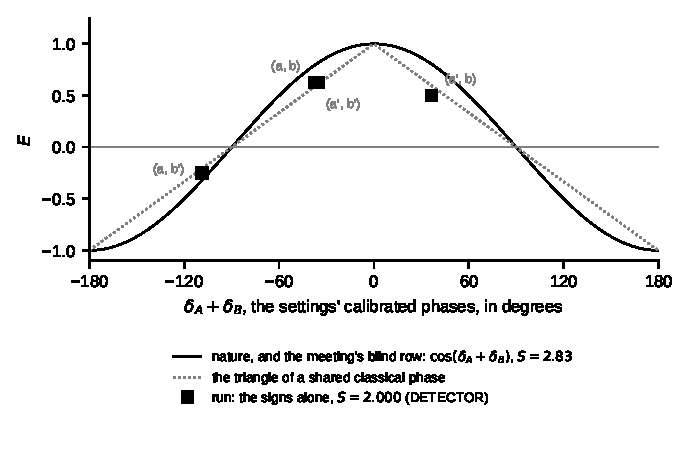
\includegraphics[width=0.72\linewidth]{figures/bell.pdf}\caption{\label{fig:bell}Bell: the correlation $E$ at the four settings against the sum of the settings' calibrated phases, the run with side B credited by the contrast (the filled marks, \textsc{detector}) and the run by the signs alone on both sides (the open marks), beside nature's $\cos(\delta_A + \delta_B)$ and the triangle of a shared classical phase read by its sign. The filled marks follow the cosine at the efficiency $0.64$; the open marks, every quantum credited, follow the triangle and sum to $S = 2.000$. Drawn from the rows of the law's document; no run of this paper's.}\end{figure}

\paragraph{The two numbers, and where the law and nature part.} By the signs alone on both sides, every quantum credited, the efficiency $1$ and $1$: $S = 2.000$ to three places, the triangle's identity and not a coincidence of angles (with both outcomes the sign of $\cos(u - \delta)$, $E$ is the sawtooth $1 - 2\,|\delta_A + \delta_B| / \pi$, and the CHSH sum of a sawtooth is exactly $2$ for every ordered set of four settings within one period), the cleanest check that the board is local and the pair's phase a shared classical variable. By B's credit by the contrast, the efficiency $1$ and $0.64$: $S = 2.76$ among the coincidences, nature's $E = \cos(\delta_A + \delta_B)$ reproduced through the instrument's declaration, the credited sample depending on the pair's phase and the setting. The excess from $2$ to $2.76$ is the detection loophole and nothing else (\claimmark{derived}, the advisor's theorem: any rule in which A's credit depends on $(a, u)$ and B's on $(b, u)$, deterministic or drawn, with every pair counted, gives at most $2$). So the law's row matches the coincidence correlations of every Bell experiment whose detection efficiency is below the loophole's bound, all of them before 2015, and predicts no violation once the loophole is closed; nature's loophole-free runs of 2015, photons above $2 / 3$ and event-ready spins, at efficiencies above $0.83$, still saw $2.4$ to $2.8$; there, and only there, the law and nature part. No other road: a joint credit reading both settings is closed by the owner's word (no reading together, two detectors are never at one Node; the opposite events written at A go forward from A and never reach B, and even declared backward would arrive late by $2L\sqrt 3$ intervals); a pair amplitude is not on the board; settings chosen by the board's own past have no mechanism. Two findings on the design, kept in the row and no rows: the first near-field run at $L = 2d$ with the gaps five wide, whose comb flipped the larger port at the wrong $u$ and gave $S = 2.09$ with a curve that is not the algebra's, no finding either way; and the far-field design (the gaps of three rows at $d = 8$, $L = 48$, the spacing $48$ on a board of $96$ rows), through whose gaps the light left into the whole half-plane, the screens seeing $4.8$ percent of the quanta and the run ending at the $y$ face's largest size. The superdeterministic world, the settings set by bodies on the board that share the source's history, is a world under its own name and not before this one: two detectors on one board correlated before the click lie inside Bell's $\lambda$ and do not raise the bound, which falls only to the settings inside $\lambda$ or to a non-local click \cite[the rows against nature, (h)]{algebra}\cite[Bell by the detector's contrast, the two slits as designed]{decisions}.

\section{The constants, and what is open}\label{sec:constants}

\subsection{The constants}\label{sec:constants-law}

The causal bound is one Link per interval, and light's own speed at long wavelength is $1 / \sqrt 3$ Links per interval (Section~\ref{sec:line}). The quantum of action is one click, its energy the quantum's norm $T$ of its family. The quantum of distance is the Link, of time the interval; nothing between two Nodes or two intervals is observed. Newton's constant is not declared: a body whose wells are $s$ quanta per interval makes the massless row's rest $3\,G(r)\,s$ at $r$ Links over the row's divisor, $0.7582\,s$ at the Node and $3s / (4\pi r)$ far away, and the level slows the clock by the potential $\Phi = -c / \Gamma$, so (\claimmark{derived})
\begin{equation}\label{eq:G}
G = \frac{3}{4\pi\,\Gamma\,E_g} \text{ per quantum of well, in Links and intervals},
\end{equation}
a reading of $\Gamma$, the file's $E_g$ and the lattice, and no number of the law; a world at a smaller $\Gamma$ has stronger gravity per unit of content, and the ratios between rows carry $G$ once and cancel it. The row's source moves by whole quanta of well and never by less, and the field itself is no click. The vacuum content, the massless row's declared rest, is the law's cosmological constant, $0$ by nature's clicks (Section~\ref{sec:vacuum}) \cite[the constants]{algebra}.

\paragraph{The free numbers.} Under every divisor $1$, $G$ and $\alpha$ are no numbers of the law but readings of $\Gamma$ and the GameBoard's geometry; under the two rows the file holds gravity's $E_g$ beside $\Gamma$, $T$ and the matter pair's $m$, the binding holder's gapped pair (its range $R$ tied to $\Gamma$ by the proton) and the vacuum content, $0$ by the declaration. $\Gamma$ is free and large against a proton's count, as nature's Link is small against a proton, and no ratio fixes it yet (item 19 below); $\alpha$ stays a reading; $m$ is the one integer of nature beside them, bounded by the band and the reach \cite[no free number but the mass]{algebra}.

\paragraph{$T$ is physical through $\sqrt T / \Gamma$.} $T$ is not the resolution only, though the rounding's floor stays ($2^{19}$ for a hundredth of a quantum per unit at the pixel): the level of one quantum of light is $\sqrt T / \sin\omega$, from $b^2\sin^2\omega / T = 1$, and the pace reads levels, so light's action per quantum on a body's content is $\sqrt T / (\Gamma\sin\omega_L)$, $0.07$ of $\Gamma$ for one quantum per Node at $\lambda = 8$ at $T = 2^{15}$ and $\Gamma = 6{,}000$ ($0.03$ the floor at the shortest waves, $0.28$ at $T = 2^{19}$); matter's well per quantum is $0.76$ levels, so at these $T$ and $\Gamma$ light acts on a pace $550$ times more per quantum than matter's gravity. The pair $(T, \Gamma)$ holds one physical number, $\sqrt T / \Gamma$, light's coupling per quantum, and nature's is small; what fixes it is open beside $\Gamma$ \cite[what is open, item 9]{algebra}.

\subsection{The constants the law derives with no free number}\label{sec:candidates}

A constant of nature is derived as a dimensionless number, or as a dimensional one once the units are fixed from nature; five candidates, in the order of their computation, each written before its run and each written as it comes, against nature or not \cite[the rows against nature, (v)]{algebra}:

\begin{enumerate}[leftmargin=1.6em]
\item[(1)] \emph{The bending factor of light}, the bending over the clock's share, Einstein's $2$ against Newton's $1$: $1.9$ on the lattice in the first approximation (Section~\ref{sec:forms}, (b)); the lattice computation to three digits is the first proof-grade number, $2.00$ within the rounding the direction confirmed (\claimmark{computed} in the first approximation).
\item[(2)] \emph{The strength of gravity against the quantum}, $G m^2 / (\hbar c)$: under every divisor $1$ the coupling of one quantum to another through the content holder is of order one, against nature's $1.75 \times 10^{-45}$ for the electron and $5.9 \times 10^{-39}$ for the proton, and the same number read between two charged clouds is the hierarchy (Section~\ref{sec:tworows}); decided as the two rows with the caveat, the hierarchy the file's one number, $E_g$ about $3 \times 10^{42}$ for nature, and the charged cloud look reads it as $E_g / 1{,}836^2$; the reading of scale beside it, structural within Rule3 with the well as the binding by the second family's study (Section~\ref{sec:branches}), written only from the scattering look (\claimmark{computed} under every divisor $1$; \claimmark{assumption} under the two rows).
\item[(3)] \emph{The fine-structure constant}, $\alpha$: the sign holder's well of one quantum with the sense against the content holder's well of one quantum, both at the divisor $1$, the electric against the gravitational pull between two electrons, nature's $4.2 \times 10^{42}$, and $\alpha$ itself as light's coupling to the charge, to compute, with its distance from $1 / 137.036$ (open).
\item[(4)] \emph{The mass ratio} $m_p / m_e = 1{,}836$ is the count's ratio of a cloud to one quantum, an input and not derived (Section~\ref{sec:branches}), and fixes no $\Gamma$, so (1), (2) and (3) are computed as functions of $\Gamma$ until the line that fixes it is written.
\item[(5)] \emph{The lattice constants}, $3\,G(0) = 0.7582$, $3 / (4\pi)$ far away and light's $1 / \sqrt 3$ Links per interval, the six Ports' own, exact and not nature's, entering every derivation above (\claimmark{computed}).
\end{enumerate}

\subsection{The hypotheses under their own names}\label{sec:hypotheses}

Every hypothesis stands outside the law under its own name until it passes the three tests or the owner admits it; each says what would decide it \cite[the hypotheses under their own names]{algebra}.

\begin{hypothesis}[the conversion, the weak force]\label{hyp:conversion}
A click that takes a quantum of one family and gives it as quanta of others, the rotations adding, is the whole weak interaction, one Node's act, no field and no massive vector, and no family's row declares anything for it.
\end{hypothesis}

\begin{hypothesis}[Gamma is not constant]\label{hyp:gamma}
$\Gamma_{t+1} = \Gamma_t + 6$, the step the six Ports of a Node and no free number; the rule's physics depends on the ratios $c / \Gamma$ and $m / \Gamma$ alone, so every pair steps with $\Gamma$ and the wall and the amplitude unit are derived from $\Gamma_t$ each interval; a pixel of a fixed count falls under the rising edge and dissolves, the distinct bound counts grow with $\Gamma$, light does not drift while the clocks of pixels do, the rule's Hubble rate $H = (6 / \Gamma)\,|d\ln\omega_b / d\ln(c / \Gamma)|$, and $\Gamma = 6t$ reads the universe's age in intervals. The time road's price: a stepping $\Gamma$ is Dirac's road, $G$ falling as $1 / \mathrm{age}$; nature bounds $G$'s drift today under $10^{-13}$ per year against $7 \times 10^{-11}$ per year for a $G$ proportional to $1 / \mathrm{age}$, and in the law a coupling that decays weakens the bodies' binding with it unless the binding is a row of its own, which the two rows made it \cite[Gamma is not constant]{algebra}.
\end{hypothesis}

\begin{hypothesis}[the three distances are the rule's]\label{hyp:distances}
That $\alpha$, $m_e / m_P$ and $m_p / m_e$ are derived; the algebra is closed on one root, two named assumptions, one assumption of the universe and one hypothesis, with no number but gravity's $E_g$, and is not closed toward nature by name \cite[the tree]{algebra}.
\end{hypothesis}

\begin{hypothesis}[the hill holds the body]\label{hyp:hill}
A body stands as a stable extended fixed point where a held row read with the opposite sign, of reach shorter than the hollow's, is held beside the hollow: below the hill's reach both are Coulomb-like and the hill forbids the collapse, between the two reaches the hollow binds, and the body's size lies between the reaches. Decided by a run of the generator with the third row.
\end{hypothesis}

\begin{hypothesis}[the cooling]\label{hyp:cooling}
A body above its minimum sheds its excess as quanta of its own family, messages of matter, and radiates light by its write while it breathes, the shedding stopping at the stable body theorem's minimum for its count; the engine sheds by the count's line alone, and whether a body settles at the minimum is a run's finding. The number of quanta a cloud gives to settle: for a Gaussian cloud twice too wide in its own massless well, $13$ percent leave on a chain, $20$ on a plane, $23$ in a box (\claimmark{derived}, a blind expectation) \cite[the number of quanta a cloud gives to settle]{algebra}.
\end{hypothesis}

\begin{hypothesis}[the anti-body is the sign of its quanta reversed]\label{hyp:antibody}
The anti-body of any body is the same record with its quanta of the opposite sign at its Nodes; a neutron and an antineutron are both real records and differ by that sign, the baryon number's. Decided by the owner's word of 2026-09-30 as the count's sign reversed, a lay of $-1$ moved by the count's line; with that line gone (Section~\ref{sec:left}) its restatement on the record alone is the documents' to give, and it stands here under its own name until then, read by a lay of such a body and its clicks against nature's antineutron, distinct from the neutron.
\end{hypothesis}

\begin{hypothesis}[the second level's amplitude is a count of its own]\label{hyp:charge-unit}
The second level's amplitude quantised as a count of its own, a circular quantum the unit and a body's charge its number of circular quanta, so that $|q_p| = |q_e|$ would be derived where the law as written leaves a body's charge continuous (Section~\ref{sec:sign}); no line of the law as written does it and Theorem~\ref{th:acts} may not allow it.
\end{hypothesis}

Beside them, by name: the third way of gravity (the massless row's level as a count of resting clicks relaxed each interval, which trades the exact inverse or the causality; Le Sage's shadow refused, the drag on a moving body and the absorbers' growth), a controlled phase of order one between two records (which Theorem~\ref{th:acts} excludes from the acts alone), and a cross-axis read or a current's read (frame dragging, the induction), which Rule3's line reads nowhere \cite[the fork, decided; what is open, item 15]{algebra}.

\subsection{What is open, and what is not claimed}\label{sec:open}

The law's document keeps its open items by name; an item the law's own words closed stays as one line saying why, a decided line stands against nature until tested, and a line decided with a reservation stands until one of its reopeners \cite[what is open]{algebra}.

\begin{enumerate}[leftmargin=1.6em]
\item[1 to 3.] \emph{The proton and the electron, the two branches, the fall and $Q / M$}, closed: the body of nature is the cloud, its three masses one, the proton a cloud of $1{,}836$ and the electron one quantum, $m_p / m_e$ the count's ratio fixing no $\Gamma$; the proton's size stands beside it, a body never smaller than its quanta's Compton length where nature's proton is $460$ times smaller, written from the scattering look; the coupling through the pace is universal and the response is the mode's own, so the equivalence principle holds for the bodies of nature and not for collapsed matter, whose fall is the fall look's blind row at detectors; the universality is one family's (Sections~\ref{sec:branches} and~\ref{sec:forms}).
\item[4.] \emph{The lone quantum's detection}, decided: the click ends nothing, and the detector is a declared instrument whose credit is the instrument's, so exclusivity and Born's rule are a declaration and no finding of the law, the two slits' dilute world rising click by click by the declaration (Section~\ref{sec:price}); the count's line and the sense's line, under which the item was first written, left the law (Section~\ref{sec:left}), and the algebra of the exclusivity stands in the documents under its own name.
\item[5 to 8.] \emph{The colours and the third}, closed as absent; \emph{the universe expands}, closed as a statement about boards (a board closed on every axis has no rest and its level drifts, the finite board's word); \emph{the unread parts}, closed as out; \emph{the builds}, closed as decisions.
\item[9.] \emph{$\Gamma$ and $T$}: $\Gamma$ the one scale of the law, as the Planck length is nature's, free and large against a proton's count; $T$ physical through $\sqrt T / \Gamma$; what fixes either is open.
\item[10 to 12.] \emph{Radiation reaction}, closed by the sense's build (whether a breathing body cools is a run's finding); \emph{the mass defect}, closed as the law's reading (Section~\ref{sec:stable}); \emph{the neutron and the antineutron}, closed by the sign of the quanta (Hypothesis~\ref{hyp:antibody}).
\item[13, 14.] \emph{The generator's branch and the start's sources}: the start sourced by the wells, the fixed point of the wells under the rest they make, is the pixel round's line; \emph{the tensions' start}: the start sources the time parts alone, so the tensions start at $0$ and ring up to their rest over the first intervals, a transient that is no wave of the body.
\item[15.] \emph{A cross-axis read or a current's read}, a hypothesis under its own name.
\item[16 to 18.] Whether a body at rest jitters when its current's swing reaches $T / 2$ (on sixteen Nodes the swing over $400$ intervals is one percent of $T / 2$); the self-source's cubic term, not in the engine; the stable body theorem's Hessian beyond the dilation for a set of held rows and the functional beyond first order, and whether the hill holds the body and the cooling brings a body to it, a run's findings.
\item[19.] \emph{What fixes $\Gamma$}: the mass ratio of clouds is a count's ratio and fixes no $\Gamma$; the constants of Section~\ref{sec:candidates} are computed as functions of it until the line that fixes it is written; that line is open.
\item[20.] \emph{The hierarchy of gravity and electricity}, decided with a reservation (Section~\ref{sec:tworows}): the finding of every divisor $1$ kept as the law's word on the road not taken; the reopeners the three tests, the bodies not standing under the screened sum, the charged cloud look reading nature's other way, and the finding of scale.
\item[21.] \emph{The laid row's inverse}, decided: a held row laid each interval from the wells has no whole-run inverse (the paces of an interval read a level that is a function of a level no later state holds), so every holder of the file steps by Rule3 at its pair and inverts by its own direction, and the whole run goes back in time (Section~\ref{sec:interval}).
\item[22.] \emph{The vacuum content}, decided: $0$, a declaration fixed by nature's clicks (Section~\ref{sec:vacuum}).
\item[23.] \emph{Gravitational waves and the lattice's rotations}, a finding against nature with its look: under the tension's diagonal alone the massless row's travelling events carry the breathing polarisation and the lattice-aligned $+$ polarisation only, and no $\times$, where nature's gravitational waves come in $+$ and $\times$ at every orientation; and the lattice's $48$ symmetries stand against nature's rotations at short wavelengths, light's band along an axis against the diagonal anisotropic by about $1$ percent at $\lambda = 8$ Links and tens of percent at $\lambda = 4$, falling as $(\mathrm{Link} / \lambda)^2$, a finding where nature's wavelengths are short in Links and otherwise a bound on the Link from nature's isotropy. Settled by the blind anisotropy from the band, the bound on the Link, whether a rotating source radiates on the lattice without the off-diagonal parts and what its events carry against nature's quadrupole, and a run of a rotating or breathing source on an open board with the massless row read along an axis and a diagonal, its blind row written first.
\end{enumerate}

\subsection{Nature's numbers enter the board only as clicks: the calibration series}\label{sec:calibration}

Every measured number of an experiment (a frequency, a wavelength, a deflection angle, a redshift, a coincidence rate) is first written as a click pattern on a declared detector against a declared clock and only then set beside the board's click pattern; the families' coefficients (the pairs) and the units ($\Gamma$ and $T$, what in nature is one Link and one interval, the one calibration the law does not derive) are fixed by that match and by nothing read off the board; the two ratios the law fixes without it are light's speed $1 / \sqrt 3$ Links per interval and the causal bound $1$ (\claimmark{assumption}, the owner's word of 2026-09-30) \cite[the reading, nature's numbers enter the board only as clicks]{algebra}\cite[the two slits as run are the click experiment; the experiments needed]{decisions}. What the calibration needs, each a declaration of the file or of the reading and none a number of the engine: the units; the families (which of nature's clicks belong to which row, a click reporting its family, its region and its Ports); the emitter (nature's source as a declared lay of events, or a body's write); the detector (the declared region, its credit rule, what it reports and what it does not; nature's detector efficiency and dead time the same kind of declaration); the geometry in Links, the receding face for an open laboratory; and the reading (the histogram per region, the comb, the coincidence window, applied to nature's data the same way). The advisor's reading per quantity, marked as his: a clock of nature is a click rate, a length a click's place on a screen, an energy or a mass a count of quanta, and a family's pair sets its rest rotation $\cos\omega_0 = \num / \den$, so one click rate of nature per family fixes its pair once $\Gamma$ and $T$ fix the unit. The series, one number of the law against one click pattern of nature per line, light-only meaning the engine as it is:

\begin{enumerate}[leftmargin=1.6em]
\item[(1)] \emph{The two speeds}, run as a look: the massless row's own events step at the pace $1$ at the speed $1 / \sqrt 3$ and light reads the vacuum content $x = c_{\mathrm{vac}} / \Gamma$ into its pace at $(1 - 2x) / \sqrt 3$; three worlds of one design on a board $520 \times 48$ with both $x$ faces receding, a plane packet at $k = \pi / 4$ over every row and a far region $458$ Links away: light at the content $60$, light at no content and the massless row's kick alone; the arrivals read as the centroid of each packet's bump over the region, a GameBoard reading labelled so beside light's clicks there ($1{,}200$ and $960$); light at no content before light at the content by $21.3$ intervals at the centroids and $17.0$ at the onsets against the blind $17.9$ and $17.5$ from the two bands exactly, the kick and light at no content together within $5$ intervals against the blind $0$; the gate \textsc{match} over $120$ intervals. Nature's clicks: GW170817, $|\delta c / c|$ below $10^{-15}$, which fix $c_{\mathrm{vac}} = 0$ (Section~\ref{sec:vacuum}). Beside it, (1b) \emph{gravity's divisor bounded from below by light's own fringes}: at $E_g = 1{,}000$ a packet of $1{,}333$ laid a well of $1{,}870$ levels and its paces varied by tens of percent, a self-focusing that nature never shows, since nature's fringes do not move with the intensity at any laser's power; so $E_g$ is at least the packet's summed well over one level for the strongest light ever measured, and the look is the two slits' bright world at rising amplitudes, the fringes' positions read per region against the intensity, written blind: they do not move until the packet's summed well reaches one level.
\item[(2)] \emph{Light's dispersion on the lattice}: along an axis $\cos\omega = (2 + \cos k) / 3$, the group speed falling as $1 - 0.083\,k^2$ ($5$ percent at $\lambda = 8$, $1.3$ at $16$, $0.08$ at $64$); the look two packets of different wavelengths laid together and two detectors, the arrival difference. Nature's clicks: photons of different energies from one gamma-ray burst arriving together, $|\delta v / c|$ below $10^{-16}$ at $1$ TeV, which bound the Link from above, $k = 2\pi\,\mathrm{Link} / \lambda_{\mathrm{TeV}}$ below $3.5 \times 10^{-8}$ per Link, so the Link below about $7 \times 10^{-27}$ metres, the first bound on $\Gamma$'s unit, the interval following from the Link and $c$ (\claimmark{computed}).
\item[(3)] \emph{Matter's two slits, de Broglie}, a matter message and no body, when the emitter lays a matter packet at the pair $[m, \Gamma]$: the band's curvature near its bottom, $\omega \approx \omega_0 + k^2 / (2m^*)$, gives $v = k / m^*$; the look reads the spacing $\lambda L / d$ and the packet's speed by two detectors' time of flight, the two clicks giving $m^*$ in Links and intervals, and nature's $h / (mv)$ with the units of (1) and (2) gives $m$, the matter pair.
\item[(4)] \emph{The light clock}, light-only, now: a packet between two mirror faces, the period $2L\sqrt 3$ intervals as clicks at one face's detector, a clock with no body; in a declared static well of the massless row its rate falls by $x$ and a screen beside it reads the bending $2x$, the Einstein rows of Section~\ref{sec:forms} as clicks with the ratio $2$ blind; $E_g$ enters only when the well is sourced by a body and waits with the pixel.
\item[(5)] \emph{The binding pair and $E_g$ through bodies}, parked with the pixel.
\item[(6)] \emph{The vacuum content by light's speed alone fixes nothing}: nature defines the metre by $c$, and one speed calibrates no unit; $c_{\mathrm{vac}}$ is fixed by (1).
\end{enumerate}

\noindent The order: (1), (2) and (4) now, (3) when the emitter lays a matter packet, (5) parked \cite[the reading, nature's numbers enter the board only as clicks]{algebra}.

\paragraph{What is set beside nature, in one place, by kind.} Clicks are compared with clicks, and nothing else is a finding against nature; the index the documents keep is read by that rule \cite[only clicks against clicks]{decisions}. \emph{Click rows read}: the two slits' fringes per declared detector at the near field's places, $284$ against the blind $273$, the match (Section~\ref{sec:slits-result}); the closed gap's one-gap envelope, nature's row with the slit closed; the dilute world's pattern by the declaration, no finding either way; Bell's $E = \cos(\delta_A + \delta_B)$ and $S = 2.76$ at the detector's efficiency $0.64$, nature's coincidence correlations below the loophole's bound, and $S = 2.00$ with every quantum counted, the law's word against nature's loophole-free runs (Section~\ref{sec:bell-result}). \emph{A number fixed by nature's clicks}: the vacuum content, $0$, by GW170817 through the two speeds' look (Section~\ref{sec:vacuum}); the Link bounded below $7 \times 10^{-27}$ metres by the dispersion of a burst's photons (item (2) above), a bound and no number yet. \emph{The documents' looks with their click rows, not experiments of this paper}, each a claim of the law beside nature's click pattern, written only when its rises are in: the bending of a packet past a pixel against the clock's share at the same Node, $2.00$ within the rounding or $1.9$ sharp; the light clock's rate in a declared well with the bending beside it; the coupling as the sign and never as $Q / M$, two bodies' deflections in one sign field; gravitational waves' polarisations and the lattice's rotations (item 23); the charge's unit, the charges of laid bodies read by their deflections; the proton against the neutron and the hierarchy, the charged cloud look; the antineutron, a body of the opposite sign and its clicks; the rotation curves and the redshifts; the proton's size, the scattering look; the compact body's fall, the fall look's rises at detectors; the resonant absorber's one click, the absorption look. \emph{Left as readings, never compared with nature}: light's speed against the causal bound (the bound is no click of nature's); the three masses along the two branches; the charged cloud against the neutral one until its look; light's self-focusing at gravity's divisor $1{,}000$, a finding by name that bounds $E_g$ (item (1b) above).

\paragraph{What advancing the paper needs.} Everything nature measures is clicks, and every number of the law is a number of a file: the Node clock $\Gamma$, the quantum's action $T$, the matter pair's $m$, the binding holder's pair, gravity's divisor $E_g$, the vacuum content, and the families themselves, each a row (Section~\ref{sec:universe}). Between the two there is no dictionary yet: the paper does not know how a click pattern of nature's is turned into the file's numbers and rows, which family of the law a pattern names and at which parameters, and the rows against nature of Section~\ref{sec:forms} are read at the looks' numbers and not at nature's. Advancing the paper therefore needs specific experiments designed for that translation and for nothing else (the owner's word, 2026-09-30): for each number of the file, a click pattern of nature's whose form fixes it, read against the law's blind row at that number, and for each family the click pattern that names it, its clicks' family and axis, its band by de Broglie's row, its holding by the fields it sources. The series above is that list; its first number is fixed, the vacuum content, and its second bounded, the Link. Until the rest are named, run and read, the law's numbers are the looks' and not nature's, its families are the rule's bands and not nature's particles, and what fixes $\Gamma$ and $\sqrt T / \Gamma$ stays open; the two experiments of this paper are the first two of that series.

\paragraph{Not claimed.} Any agreement with nature beyond the rows shown: the two slits' fringes and the closed gap's envelope, and Bell's coincidence correlations at the detector's efficiency $0.64$; that nature is so; the Lorentz group, which is no symmetry of the lattice; a mechanism of the click; Bell's violation at a fair sample, which no local line of the law reaches; a controlled phase of order one between two records; the fine-structure constant, the mass ratio and what fixes $\Gamma$; the spin $1/2$; the count of gravitational levels, which is the universe's history; a body's settling, which is the hypothesis of the cooling. Every hypothesis of the paper is named as one.

\section{The engine that computes it}\label{sec:engine}

The engine, Universe24 \cite{zenodo}\cite{engine}, is the law's implementation and nothing else: a GameBoard of Nodes, every family's NodeState at every Node, and one interval of acts in the law's order, each a call of Rule3 on whole-board arrays in $64$-bit integers, every neighbour read through a Port. It holds no number, no formula, no family's name and no flag; every physical value comes from the run's files; no act of the interval takes a square root and no act reads a Node to decide anything. It is seven modules under $400$ lines each (the Node's acts, the lay, the flows into a held row's tensions, the reports, the receding face's growth, the GameBoard that walks the interval forward and back, and the files with their loader) on a core of Rule3, the Ports and the working bound; every family is a row of the universe file found by its name, and a new family is a row and no code. The engine on \texttt{main} at this writing still carries the count's and the sense's lines with their arrays and the \texttt{click} line of the count's line, which the owner's word of 2026-10-01 removes (Section~\ref{sec:left}); under that word the measurement is the \texttt{seen} line's inflow and the reader's credit, as the rows of Section~\ref{sec:slits} already read it \cite[the engine; the NodeState; how to add a family]{engine}\cite[the genericity of the families; not one number in the engine]{decisions}.

\paragraph{The files.} \emph{The universe file} declares the integers ($\Gamma$, $T$, the width) and the families, each its name, its pair and, for a held family, what it holds, its divisor and, on the massless row, its rest; the rule derives the rest. \emph{The world file} declares the board's shape and its faces (periodic, open or closed; the inner faces with their gaps; the receding faces with their largest size and their layers per growth), the intervals, the bodies by their family, their Nodes with their counts and the quanta of other families they hold, the messages by their family, axis, wave number, amplitude, envelope, phase and transverse wave number, and the detectors by their regions or the body they name; a missing key is refused by name, and no default is written. \emph{The mode file} beside the world holds the generator's levels of every body and message. \emph{The expectation file} holds the blind row, every number the file's: the regions, the window, the blind counts and the draw's seed for a screen; the ports, the settings, the calibrated phases and the blind $E$ and $S$ for Bell. The two experiments' worlds are written by a builder from one design file each, every number of the worlds in it \cite[the loader and the files; how to run a world]{engine}.

\paragraph{A run.} The generator lays the bodies and the messages; the run is headless, one output file per world with the verdict (\textsc{lawful}, or \textsc{refused} with the reason, the guard's at load among them), the intervals run, the end where a receding face reached its largest size, one \texttt{seen} line per family and region per interval with the net current through the region's front boundary (what the instrument saw, the host's reading for the credit), a \texttt{field} line per region with a family's density over it (a GameBoard reading), and the books (a GameBoard diagnostic, the least Link pace of the final state among them). The readers: the screen's reader takes a world's \texttt{seen} lines over the window against the expectation file and gives per region the share, $N$ the total over $\Wc$, the laid count less $N$ as the part that left elsewhere, the clicks credited by the largest remainders and one draw of $N$ clicks by the shares at the declared seed, \textsc{detector}; Bell's reader takes the runs' \texttt{seen} lines per port, calibrates the ports and the settings' phases, credits side A by the sign and side B by the contrast, and gives $E$ among the coincidences, $S$, the efficiencies and the readings beside them in exact fractions; the two speeds' reader takes the \texttt{field} lines at the far region. A look runs only after the back-in-time gate says \textsc{match} on its own world over its intervals \cite[the output; how to run a world]{engine}.

\paragraph{The gates.} Every pull request runs lint, formatting, strict types and the tests of the changed files and their consumers; the gates hold the rule's arithmetic to one function, every shift across a Link to the Ports, every integer literal of the engine and its tools to the law's own, no root anywhere, every module to integers alone, the acts against Rule3 by hand, the interval on a closed cube (every holder at an isotropic rest, the $48$ symmetries in every part, the gate \textsc{match}), the tension as Rule3's own conservation of the current, light born by the write, the receding face on a chain of light alone (the run the larger chain's bit for bit, no reflection where the fixed chain reflects), the rest of every pair as its line's own fixed point, the generator's bodies and its message lay against the real numbers, the inner face's gap and reflection, the documents' headings and the repository's language. A behaviour change needs a dedicated test; a physics change starts from the law's line \cite[the gates]{engine}.

\paragraph{To test a hypothesis.} Write its line in the law's document first, under its own name, with the three verdicts; the advisor computes the blind number from the engine's own lines; the worker builds it as one pure function of arrays that calls Rule3 alone, with its test, on one short branch; the world and its blind expectation are written before the run; the run's reading is compared with that number, a difference being a defect of the engine and never a finding, and a number outside its band with no defect found naming the missing law as a hypothesis under its own name. No expectation is rewritten after a look, and no body's number is tuned to a result \cite[the blind number first]{workflow}.

\section*{Declarations}

\paragraph{Funding.} None.
\paragraph{Competing interests.} None.
\paragraph{Ethics approval, consent to participate and consent for publication.} Not applicable; no human or animal participants.
\paragraph{Data and code availability.} The law's document, the engine that computes the rule and the figures' scripts are archived at Zenodo under the concept DOI 10.5281/zenodo.22738746 \cite{zenodo}, under the MIT licence; the runs this paper cites, the two slits, Bell and the two speeds, are cited through the law's document and name their commits there.
\paragraph{Author contributions.} The author laid down every postulate and decision of the model, directed the work and wrote the paper.
\paragraph{The use of a large language model.} The author used a large language model (Claude, Anthropic, through Claude Code, 2026) extensively as a tool, under his direction and instructions, for the software, the computations, the mathematical derivations and their checks, the physics of the law's document and the drafting of the text; the model is not an author; the author reviewed and edited every statement and takes full responsibility for the content. No figure was made by a generative tool; every figure is drawn by a script from the definitions or from the documents' rows.

{\small
\begin{thebibliography}{99}
\bibitem{algebra} The law of the GameBoard, \texttt{docs/ALGEBRA.md} of the archive \cite{zenodo}, cited by the name of its section: the GameBoard and the families (the objects, a family's declaration, the interval, readings and measurements); Rule3 (the line, the direction, the four acts, the paces, the bound, the self-source, the conserved form); the click (the booking, the count's line, no click names a Node, the algebra of the exclusivity); the primitives; the stable body (what a body is, the well, the functional and the dilation, the surplus leaves, the generator, the velocity); what the law says of nature (the reading, with no waves on the event board, what produces a click is not known and nature's numbers enter the board only as clicks; the hypotheses under their own names; the postulates; the constants; the rows against nature); what is open.
\bibitem{engine} The engine, \texttt{docs/ENGINE.md} of the archive \cite{zenodo}: the words, the NodeState, the interval, the loader and the files, the output, how to run a world, how to add a family, the gates.
\bibitem{decisions} The decisions, \texttt{docs/HIGHLIGHTS.md} of the archive \cite{zenodo}: the model owner's decisions in force, one line each, cited by the line's name.
\bibitem{workflow} The shared way of working, \texttt{skills/workflow.md} of the archive \cite{zenodo}: the three tests, the six verbs, the blind number first, the short procedure.
\bibitem{zenodo} A. Gonen, Universe24: a discrete simulator of local physical laws (Reality Theory), Zenodo (2026), \url{https://doi.org/10.5281/zenodo.22738746} (the concept DOI, resolving to the latest version).
\end{thebibliography}}

\end{document}
